\documentclass[]{book}
\usepackage{lmodern}
\usepackage{amssymb,amsmath}
\usepackage{ifxetex,ifluatex}
\usepackage{fixltx2e} % provides \textsubscript
\ifnum 0\ifxetex 1\fi\ifluatex 1\fi=0 % if pdftex
  \usepackage[T1]{fontenc}
  \usepackage[utf8]{inputenc}
\else % if luatex or xelatex
  \ifxetex
    \usepackage{mathspec}
  \else
    \usepackage{fontspec}
  \fi
  \defaultfontfeatures{Ligatures=TeX,Scale=MatchLowercase}
\fi
% use upquote if available, for straight quotes in verbatim environments
\IfFileExists{upquote.sty}{\usepackage{upquote}}{}
% use microtype if available
\IfFileExists{microtype.sty}{%
\usepackage{microtype}
\UseMicrotypeSet[protrusion]{basicmath} % disable protrusion for tt fonts
}{}
\usepackage{hyperref}
\hypersetup{unicode=true,
            pdftitle={The Surgical Informatics Cookbook},
            pdfauthor={Surgical Informatics, University of Edinburgh},
            pdfborder={0 0 0},
            breaklinks=true}
\urlstyle{same}  % don't use monospace font for urls
\usepackage{natbib}
\bibliographystyle{apalike}
\usepackage{color}
\usepackage{fancyvrb}
\newcommand{\VerbBar}{|}
\newcommand{\VERB}{\Verb[commandchars=\\\{\}]}
\DefineVerbatimEnvironment{Highlighting}{Verbatim}{commandchars=\\\{\}}
% Add ',fontsize=\small' for more characters per line
\usepackage{framed}
\definecolor{shadecolor}{RGB}{248,248,248}
\newenvironment{Shaded}{\begin{snugshade}}{\end{snugshade}}
\newcommand{\AlertTok}[1]{\textcolor[rgb]{0.94,0.16,0.16}{#1}}
\newcommand{\AnnotationTok}[1]{\textcolor[rgb]{0.56,0.35,0.01}{\textbf{\textit{#1}}}}
\newcommand{\AttributeTok}[1]{\textcolor[rgb]{0.77,0.63,0.00}{#1}}
\newcommand{\BaseNTok}[1]{\textcolor[rgb]{0.00,0.00,0.81}{#1}}
\newcommand{\BuiltInTok}[1]{#1}
\newcommand{\CharTok}[1]{\textcolor[rgb]{0.31,0.60,0.02}{#1}}
\newcommand{\CommentTok}[1]{\textcolor[rgb]{0.56,0.35,0.01}{\textit{#1}}}
\newcommand{\CommentVarTok}[1]{\textcolor[rgb]{0.56,0.35,0.01}{\textbf{\textit{#1}}}}
\newcommand{\ConstantTok}[1]{\textcolor[rgb]{0.00,0.00,0.00}{#1}}
\newcommand{\ControlFlowTok}[1]{\textcolor[rgb]{0.13,0.29,0.53}{\textbf{#1}}}
\newcommand{\DataTypeTok}[1]{\textcolor[rgb]{0.13,0.29,0.53}{#1}}
\newcommand{\DecValTok}[1]{\textcolor[rgb]{0.00,0.00,0.81}{#1}}
\newcommand{\DocumentationTok}[1]{\textcolor[rgb]{0.56,0.35,0.01}{\textbf{\textit{#1}}}}
\newcommand{\ErrorTok}[1]{\textcolor[rgb]{0.64,0.00,0.00}{\textbf{#1}}}
\newcommand{\ExtensionTok}[1]{#1}
\newcommand{\FloatTok}[1]{\textcolor[rgb]{0.00,0.00,0.81}{#1}}
\newcommand{\FunctionTok}[1]{\textcolor[rgb]{0.00,0.00,0.00}{#1}}
\newcommand{\ImportTok}[1]{#1}
\newcommand{\InformationTok}[1]{\textcolor[rgb]{0.56,0.35,0.01}{\textbf{\textit{#1}}}}
\newcommand{\KeywordTok}[1]{\textcolor[rgb]{0.13,0.29,0.53}{\textbf{#1}}}
\newcommand{\NormalTok}[1]{#1}
\newcommand{\OperatorTok}[1]{\textcolor[rgb]{0.81,0.36,0.00}{\textbf{#1}}}
\newcommand{\OtherTok}[1]{\textcolor[rgb]{0.56,0.35,0.01}{#1}}
\newcommand{\PreprocessorTok}[1]{\textcolor[rgb]{0.56,0.35,0.01}{\textit{#1}}}
\newcommand{\RegionMarkerTok}[1]{#1}
\newcommand{\SpecialCharTok}[1]{\textcolor[rgb]{0.00,0.00,0.00}{#1}}
\newcommand{\SpecialStringTok}[1]{\textcolor[rgb]{0.31,0.60,0.02}{#1}}
\newcommand{\StringTok}[1]{\textcolor[rgb]{0.31,0.60,0.02}{#1}}
\newcommand{\VariableTok}[1]{\textcolor[rgb]{0.00,0.00,0.00}{#1}}
\newcommand{\VerbatimStringTok}[1]{\textcolor[rgb]{0.31,0.60,0.02}{#1}}
\newcommand{\WarningTok}[1]{\textcolor[rgb]{0.56,0.35,0.01}{\textbf{\textit{#1}}}}
\usepackage{longtable,booktabs}
\usepackage{graphicx,grffile}
\makeatletter
\def\maxwidth{\ifdim\Gin@nat@width>\linewidth\linewidth\else\Gin@nat@width\fi}
\def\maxheight{\ifdim\Gin@nat@height>\textheight\textheight\else\Gin@nat@height\fi}
\makeatother
% Scale images if necessary, so that they will not overflow the page
% margins by default, and it is still possible to overwrite the defaults
% using explicit options in \includegraphics[width, height, ...]{}
\setkeys{Gin}{width=\maxwidth,height=\maxheight,keepaspectratio}
\IfFileExists{parskip.sty}{%
\usepackage{parskip}
}{% else
\setlength{\parindent}{0pt}
\setlength{\parskip}{6pt plus 2pt minus 1pt}
}
\setlength{\emergencystretch}{3em}  % prevent overfull lines
\providecommand{\tightlist}{%
  \setlength{\itemsep}{0pt}\setlength{\parskip}{0pt}}
\setcounter{secnumdepth}{5}
% Redefines (sub)paragraphs to behave more like sections
\ifx\paragraph\undefined\else
\let\oldparagraph\paragraph
\renewcommand{\paragraph}[1]{\oldparagraph{#1}\mbox{}}
\fi
\ifx\subparagraph\undefined\else
\let\oldsubparagraph\subparagraph
\renewcommand{\subparagraph}[1]{\oldsubparagraph{#1}\mbox{}}
\fi

%%% Use protect on footnotes to avoid problems with footnotes in titles
\let\rmarkdownfootnote\footnote%
\def\footnote{\protect\rmarkdownfootnote}

%%% Change title format to be more compact
\usepackage{titling}

% Create subtitle command for use in maketitle
\providecommand{\subtitle}[1]{
  \posttitle{
    \begin{center}\large#1\end{center}
    }
}

\setlength{\droptitle}{-2em}

  \title{The Surgical Informatics Cookbook}
    \pretitle{\vspace{\droptitle}\centering\huge}
  \posttitle{\par}
    \author{Surgical Informatics, University of Edinburgh}
    \preauthor{\centering\large\emph}
  \postauthor{\par}
      \predate{\centering\large\emph}
  \postdate{\par}
    \date{2019-11-09}

\usepackage{booktabs}

\usepackage{amsthm}
\newtheorem{theorem}{Theorem}[chapter]
\newtheorem{lemma}{Lemma}[chapter]
\theoremstyle{definition}
\newtheorem{definition}{Definition}[chapter]
\newtheorem{corollary}{Corollary}[chapter]
\newtheorem{proposition}{Proposition}[chapter]
\theoremstyle{definition}
\newtheorem{example}{Example}[chapter]
\theoremstyle{definition}
\newtheorem{exercise}{Exercise}[chapter]
\theoremstyle{remark}
\newtheorem*{remark}{Remark}
\newtheorem*{solution}{Solution}
\begin{document}
\maketitle

{
\setcounter{tocdepth}{1}
\tableofcontents
}
\hypertarget{section}{%
\chapter*{}\label{section}}
\addcontentsline{toc}{chapter}{}


\includegraphics[width=30.97in]{/home/rots/cookbook/img/surgical_informatics_minibanner}

\hypertarget{intro}{%
\chapter{Introduction}\label{intro}}

\hypertarget{how-to-contribute}{%
\section{How to contribute}\label{how-to-contribute}}

(Steps 1. to 5. only need to be done once - to set-up.)

\begin{enumerate}
\def\labelenumi{\arabic{enumi}.}
\item
  Connect your RStudio and GitHub using these instructions, only up to
  ``Create new project'' is necessary here (the repository/project
  already exists):
  \url{https://www.datasurg.net/2015/07/13/rstudio-and-github/}
\item
  Get your GitHub account added to the surgicalinformatics organisation
  on GitHub (ask Riinu/Ewen):
  \url{https://github.com/SurgicalInformatics}
\item
  Open the terminal on argonaut, go to your home folder (just
  \texttt{cd} will default to taking you home). If the prompt says
  \texttt{username@argonaut:\textasciitilde{}\$} that means you're home
  - \texttt{\textasciitilde{}} means user's home.
\item
  In the terminal, do
  \texttt{git\ clone\ https://github.com/SurgicalInformatics/cookbook.git}
\item
  Look at the Files tab - a new folder called \texttt{cookbook} should
  have appeared at the bottom. Click on it and open the cookbook.Rproj
  file.
\item
  Add your thing by editing the appropriate .Rmd file - there's one for
  each chapter. In the \texttt{Build} pane (next to
  \texttt{Environment}) \textbf{click on More - Clean All} (if you don't
  do this you may be able to compile the book with code that won't work
  at a subsequent clean build which can be trickier to debug). Use the
  Build tab to Build your changes into a book.
\item
  If anyone has pushed since you cloned/last pulled (hopefully they've
  not been working on the exact same chapter): Make sure you
  \textbf{click on More - Clean All} (as above). Then Pull from the Git
  tab. This only cleans the output files - html and PDF, it will not
  touch the changes you've made in the .Rmd file.
\item
  Then Build Book again - this will include the new changes you pulled
  as well as your changes.
\item
  Git tab - commit everything, Push quickly before anyone else does or
  you'll have to go back to step 7. You can check for new pushed commits
  here:
  \url{https://github.com/SurgicalInformatics/cookbook/commits/master}
  Alternatively there's no harm in clicking the Pull button again - it
  should then say ``Already up-to-date''.
\end{enumerate}

\begin{quote}
Pro tip: instead of clicking on every single file in the Git tab, go to
the terminal, \texttt{cd\ cookbook} to go to the project folder if still
home, and do \texttt{git\ add\ -A} which is the same thing. Still need
to Commit though!
\end{quote}

\textbf{10. Have fun!}

\hypertarget{rules-of-posting}{%
\section{Rules of posting}\label{rules-of-posting}}

Rules of how to post here.

\hypertarget{indexing}{%
\section{Indexing}\label{indexing}}

\hypertarget{index}{%
\subsection{Index}\label{index}}

Bold index headings:\\
\texttt{\textbackslash{}index\{linear\ regression@\textbackslash{}textbf\{linear\ regression\}\}}
(ticks in .Rmd file are excluded when actually using)

Sub-entries of bold headings:\\
\texttt{\textbackslash{}index\{linear\ regression@\textbackslash{}textbf\{linear\ regression\}!diagnostics\}}

Stand-alone entries:\\
\texttt{\textbackslash{}index\{linear\ regression\}}

\hypertarget{chapter-and-section-references}{%
\subsection{Chapter and section
references}\label{chapter-and-section-references}}

You can label chapter and section titles using \texttt{\{\#label\}}
after them, e.g., we can reference Chapter
\texttt{\textbackslash{}@ref(intro)} (ticks in .Rmd are excluded when
actually using). If you do not manually label them, there will be
automatic labels anyway, e.g., Chapter
\texttt{\textbackslash{}@ref(methods)}.

\hypertarget{figure-and-table-references}{%
\subsection{Figure and table
references}\label{figure-and-table-references}}

Figures and tables with captions will be placed in \texttt{figure} and
\texttt{table} environments, respectively.

\begin{Shaded}
\begin{Highlighting}[]
\KeywordTok{par}\NormalTok{(}\DataTypeTok{mar =} \KeywordTok{c}\NormalTok{(}\DecValTok{4}\NormalTok{, }\DecValTok{4}\NormalTok{, }\FloatTok{.1}\NormalTok{, }\FloatTok{.1}\NormalTok{))}
\KeywordTok{plot}\NormalTok{(pressure, }\DataTypeTok{type =} \StringTok{'b'}\NormalTok{, }\DataTypeTok{pch =} \DecValTok{19}\NormalTok{)}
\end{Highlighting}
\end{Shaded}

\begin{figure}

{\centering 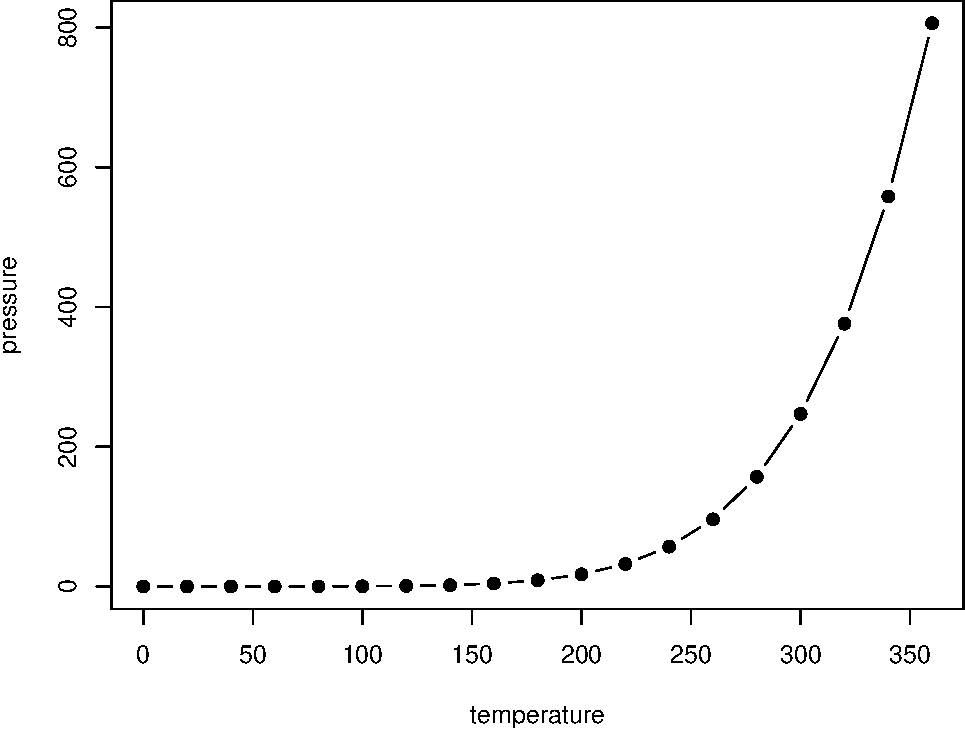
\includegraphics[width=0.8\linewidth]{cookbook_files/figure-latex/nice-fig-1} 

}

\caption{Here is a nice figure!}\label{fig:nice-fig}
\end{figure}

Reference a figure by its code chunk label with the \texttt{fig:}
prefix, e.g., see Figure \texttt{\textbackslash{}@ref(fig:nice-fig)}.
Similarly, you can reference tables generated from
\texttt{knitr::kable()}, e.g., see Table
\texttt{\textbackslash{}@ref(tab:nice-tab)}.

\begin{Shaded}
\begin{Highlighting}[]
\NormalTok{knitr}\OperatorTok{::}\KeywordTok{kable}\NormalTok{(}
  \KeywordTok{head}\NormalTok{(iris, }\DecValTok{20}\NormalTok{), }\DataTypeTok{caption =} \StringTok{'Here is a nice table!'}\NormalTok{,}
  \DataTypeTok{booktabs =} \OtherTok{TRUE}
\NormalTok{)}
\end{Highlighting}
\end{Shaded}

\begin{table}[t]

\caption{\label{tab:nice-tab}Here is a nice table!}
\centering
\begin{tabular}{rrrrl}
\toprule
Sepal.Length & Sepal.Width & Petal.Length & Petal.Width & Species\\
\midrule
5.1 & 3.5 & 1.4 & 0.2 & setosa\\
4.9 & 3.0 & 1.4 & 0.2 & setosa\\
4.7 & 3.2 & 1.3 & 0.2 & setosa\\
4.6 & 3.1 & 1.5 & 0.2 & setosa\\
5.0 & 3.6 & 1.4 & 0.2 & setosa\\
\addlinespace
5.4 & 3.9 & 1.7 & 0.4 & setosa\\
4.6 & 3.4 & 1.4 & 0.3 & setosa\\
5.0 & 3.4 & 1.5 & 0.2 & setosa\\
4.4 & 2.9 & 1.4 & 0.2 & setosa\\
4.9 & 3.1 & 1.5 & 0.1 & setosa\\
\addlinespace
5.4 & 3.7 & 1.5 & 0.2 & setosa\\
4.8 & 3.4 & 1.6 & 0.2 & setosa\\
4.8 & 3.0 & 1.4 & 0.1 & setosa\\
4.3 & 3.0 & 1.1 & 0.1 & setosa\\
5.8 & 4.0 & 1.2 & 0.2 & setosa\\
\addlinespace
5.7 & 4.4 & 1.5 & 0.4 & setosa\\
5.4 & 3.9 & 1.3 & 0.4 & setosa\\
5.1 & 3.5 & 1.4 & 0.3 & setosa\\
5.7 & 3.8 & 1.7 & 0.3 & setosa\\
5.1 & 3.8 & 1.5 & 0.3 & setosa\\
\bottomrule
\end{tabular}
\end{table}

\hypertarget{citations}{%
\subsection{Citations}\label{citations}}

You can write citations, too. For example, we are using the
\textbf{bookdown} package \citep{R-bookdown} in this sample book, which
was built on top of R Markdown and \textbf{knitr} \citep{xie2015}.

\hypertarget{snippets}{%
\chapter{Snippets}\label{snippets}}

Random useful snippets that do not fit anywhere else.

\hypertarget{creating-reproducible-r-examples-to-share-in-the-group-binder-holepunch-and-docker}{%
\section{Creating Reproducible R Examples to Share in the Group (binder,
holepunch and
docker)}\label{creating-reproducible-r-examples-to-share-in-the-group-binder-holepunch-and-docker}}

When asking for help with R code having a reproducible example is
crucial (some mock data that others can use along with your code to
reproduce your error). Often this can be done easily with creation of a
small tibble and posting of the code on slack but sometimes it requires
more complex data or the error is due to something in the Linux system
in which RStudio server is hosted. For example if the \texttt{cairo}
package for Linux isn't installed then plots don't work. The
\texttt{holepunch} package helps to reproduce examples like these (not
suitable for projects with confidential data).

\hypertarget{create-basic-reproducible-examples}{%
\subsection{Create Basic Reproducible
Examples}\label{create-basic-reproducible-examples}}

The three main parts of the reproducible example (reprex) in Surgical
Informatics are 1. packages, 2. small dataset and 3. code. Other things
like R version and Linux version can be assumed as we all use one of
only a few servers.

If you have a small (and confidential) set of data in a tibble or data
frame called \texttt{my\_data} and want it to be easily copied run:
\texttt{dput(droplevels(my\_data))}. This will print out code in the
console that can be copy-pasted to reproduce the data frame.
Alternatively use the \texttt{tibble} or \texttt{tribble} functions to
create it from scratch (this is preferable for simple datasets). Then
copy in the packages and finally the code (ideally the least amount
possible to generate the error) and share with the group e.g.:

\begin{Shaded}
\begin{Highlighting}[]
\KeywordTok{library}\NormalTok{(tidyverse)}

\CommentTok{# Output generated from dput(droplevels(my_data))}
\NormalTok{data =}\StringTok{ }\KeywordTok{structure}\NormalTok{(}\KeywordTok{list}\NormalTok{(}\DataTypeTok{a =} \KeywordTok{c}\NormalTok{(}\DecValTok{1}\NormalTok{, }\DecValTok{2}\NormalTok{, }\DecValTok{3}\NormalTok{), }\DataTypeTok{b =} \KeywordTok{c}\NormalTok{(}\StringTok{"a"}\NormalTok{, }\StringTok{"b"}\NormalTok{, }\StringTok{"c"}\NormalTok{), }\DataTypeTok{c =} \DecValTok{10}\OperatorTok{:}\DecValTok{12}\NormalTok{), }\DataTypeTok{.Names =} \KeywordTok{c}\NormalTok{(}\StringTok{"a"}\NormalTok{, }
\StringTok{"b"}\NormalTok{, }\StringTok{"c"}\NormalTok{), }\DataTypeTok{row.names =} \KeywordTok{c}\NormalTok{(}\OtherTok{NA}\NormalTok{, }\OperatorTok{-}\NormalTok{3L), }\DataTypeTok{class =} \KeywordTok{c}\NormalTok{(}\StringTok{"tbl_df"}\NormalTok{, }\StringTok{"tbl"}\NormalTok{, }
\StringTok{"data.frame"}\NormalTok{))}

\NormalTok{data }\OperatorTok\StringTok{ }
\StringTok{  }\KeywordTok{mutate}\NormalTok{(}\DataTypeTok{newvar =}\NormalTok{ a }\OperatorTok{/}\NormalTok{b)}
\end{Highlighting}
\end{Shaded}

\begin{verbatim}
## Error: Evaluation error: non-numeric argument to binary operator.
\end{verbatim}

\hypertarget{holepunch---complex-reproducible-examples}{%
\subsection{\texorpdfstring{\texttt{holepunch} - Complex Reproducible
Examples}{holepunch - Complex Reproducible Examples}}\label{holepunch---complex-reproducible-examples}}

From your project with data you are happy to make public make sure you
are backed up to \texttt{git} and \texttt{GitHub}. See the relevant
chapter on how to do this. Then run the following:

\begin{Shaded}
\begin{Highlighting}[]
\CommentTok{# Holepunch testing}

\NormalTok{remotes}\OperatorTok{::}\KeywordTok{install_github}\NormalTok{(}\StringTok{"karthik/holepunch"}\NormalTok{)}

\KeywordTok{library}\NormalTok{(holepunch)}
\KeywordTok{write_compendium_description}\NormalTok{(}\DataTypeTok{package =} \StringTok{"Title of my project"}\NormalTok{, }
                             \DataTypeTok{description =} \StringTok{"Rough description of project or issue"}\NormalTok{)}

\KeywordTok{write_dockerfile}\NormalTok{(}\DataTypeTok{maintainer =} \StringTok{"SurgicalInformatics"}\NormalTok{)}

\KeywordTok{generate_badge}\NormalTok{()}

\KeywordTok{build_binder}\NormalTok{()}
\end{Highlighting}
\end{Shaded}

The file will generate some text to copy into the top of a
\texttt{README.md} file. It will look like:

\begin{Shaded}
\begin{Highlighting}[]
\OperatorTok{<!--}\StringTok{ }\NormalTok{badges}\OperatorTok{:}\StringTok{ }\NormalTok{start }\OperatorTok{-}\NormalTok{->}
\NormalTok{[}\OperatorTok{!}\NormalTok{[Launch Rstudio Binder](http}\OperatorTok{:}\ErrorTok{//}\NormalTok{mybinder.org}\OperatorTok{/}\NormalTok{badge_logo.svg)](https}\OperatorTok{:}\ErrorTok{//}\NormalTok{mybinder.org}\OperatorTok{/}\NormalTok{v2}\OperatorTok{/}\NormalTok{gh}\OperatorTok{/}\NormalTok{SurgicalInformatics}\OperatorTok{/}\ErrorTok{<}\NormalTok{project}\OperatorTok{>}\ErrorTok{/}\NormalTok{master?}\DataTypeTok{urlpath=}\NormalTok{rstudio)}
\OperatorTok{<!--}\StringTok{ }\NormalTok{badges}\OperatorTok{:}\StringTok{ }\NormalTok{end }\OperatorTok{-}\NormalTok{->}
\end{Highlighting}
\end{Shaded}

Now, whenever somebody clicks on the badge in the \texttt{README} on
\texttt{GitHub} they will be taken to an RStudio server instance with
all your files (excluding files listed in \texttt{.gitignore}), all the
current versions of your package, all the current Linux packages and the
current R version. They can then test your code in an near-identical
environment to help identify the source of the error, their session will
time out after 10 minutes of inactivity or 12 hours since starting and
will not save anything so should only be used for bug-testing or quick
examples.

As this is a free version of RStudio server there is a limit to what is
supported and it shouldn't be used for computationally-intensive
processes.

And, as mentioned: \textbf{No confidential data.}

\hypertarget{working-with-chis}{%
\section{Working with CHIs}\label{working-with-chis}}

Here are 4 functions for CHIs that could even be put in a small package.
The Community Health Index (CHI) is a population register, which is used
in Scotland for health care purposes. The CHI number uniquely identifies
a person on the index.

\hypertarget{chi_dob---extract-date-of-birth-from-chi}{%
\subsection{\texorpdfstring{\texttt{chi\_dob()} - Extract date of birth
from
CHI}{chi\_dob() - Extract date of birth from CHI}}\label{chi_dob---extract-date-of-birth-from-chi}}

Note \texttt{cutoff\_2000}. As CHI has only a two digit year, need to
decide whether year is 1900s or 2000s. I don't think there is a formal
way of determining this.

\begin{Shaded}
\begin{Highlighting}[]
\KeywordTok{library}\NormalTok{(dplyr)}
\NormalTok{chi =}\StringTok{ }\KeywordTok{c}\NormalTok{(}\StringTok{"1009701234"}\NormalTok{, }\StringTok{"1811431232"}\NormalTok{, }\StringTok{"1304496368"}\NormalTok{)}
\CommentTok{# These CHIs are not real. }
\CommentTok{# The first is invalid, two and three are valid. }

\CommentTok{# Cut-off any thing before that number is considered 2000s}
\CommentTok{# i.e. at cutoff_2000 = 20, "18" is considered 2018, rather than 1918. }
\NormalTok{chi_dob =}\StringTok{ }\ControlFlowTok{function}\NormalTok{(.data, }\DataTypeTok{cutoff_2000 =} \DecValTok{20}\NormalTok{)\{}
\NormalTok{  .data }\OperatorTok\StringTok{ }
\StringTok{    }\NormalTok{stringr}\OperatorTok{::}\KeywordTok{str_extract}\NormalTok{(}\StringTok{".\{6\}"}\NormalTok{) }\OperatorTok\StringTok{ }
\StringTok{    }\NormalTok{lubridate}\OperatorTok{::}\KeywordTok{parse_date_time2}\NormalTok{(}\StringTok{"dmy"}\NormalTok{, }\DataTypeTok{cutoff_2000 =}\NormalTok{ cutoff_}\DecValTok{2000}\NormalTok{) }\OperatorTok\StringTok{ }
\StringTok{    }\NormalTok{lubridate}\OperatorTok{::}\KeywordTok{as_date}\NormalTok{() }\CommentTok{# Make Date object, rather than POSIXct}
\NormalTok{\}}

\KeywordTok{chi_dob}\NormalTok{(chi)}
\end{Highlighting}
\end{Shaded}

\begin{verbatim}
## [1] "1970-09-10" "1943-11-18" "1949-04-13"
\end{verbatim}

\begin{Shaded}
\begin{Highlighting}[]
\CommentTok{# From tibble}
\KeywordTok{tibble}\NormalTok{(}\DataTypeTok{chi =}\NormalTok{ chi) }\OperatorTok\StringTok{ }
\StringTok{  }\KeywordTok{mutate}\NormalTok{(}
    \DataTypeTok{dob =} \KeywordTok{chi_dob}\NormalTok{(chi)}
\NormalTok{  )}
\end{Highlighting}
\end{Shaded}

\begin{verbatim}
## # A tibble: 3 x 2
##   chi        dob       
##   <chr>      <date>    
## 1 1009701234 1970-09-10
## 2 1811431232 1943-11-18
## 3 1304496368 1949-04-13
\end{verbatim}

\hypertarget{chi_gender---extract-gender-from-chi}{%
\subsection{\texorpdfstring{\texttt{chi\_gender()} - Extract gender from
CHI}{chi\_gender() - Extract gender from CHI}}\label{chi_gender---extract-gender-from-chi}}

Ninth digit is odd for men and even for women. A test for even is
\texttt{x\ modulus\ 2\ ==\ 0}.

\begin{Shaded}
\begin{Highlighting}[]
\NormalTok{chi_gender =}\StringTok{ }\ControlFlowTok{function}\NormalTok{(.data)\{}
\NormalTok{  .data }\OperatorTok\StringTok{ }
\StringTok{    }\NormalTok{stringr}\OperatorTok{::}\KeywordTok{str_sub}\NormalTok{(}\DecValTok{9}\NormalTok{, }\DecValTok{9}\NormalTok{) }\OperatorTok\StringTok{ }
\StringTok{    }\KeywordTok{as.numeric}\NormalTok{() }\OperatorTok\StringTok{ }
\StringTok{    }\NormalTok{\{}\KeywordTok{ifelse}\NormalTok{(. }\OperatorTok\StringTok{ }\DecValTok{2} \OperatorTok{==}\StringTok{ }\DecValTok{0}\NormalTok{, }\StringTok{"Female"}\NormalTok{, }\StringTok{"Male"}\NormalTok{)\}}
\NormalTok{\}}

\KeywordTok{chi_gender}\NormalTok{(chi)}
\end{Highlighting}
\end{Shaded}

\begin{verbatim}
## [1] "Male"   "Male"   "Female"
\end{verbatim}

\begin{Shaded}
\begin{Highlighting}[]
\CommentTok{# From tibble}
\KeywordTok{tibble}\NormalTok{(}\DataTypeTok{chi =}\NormalTok{ chi) }\OperatorTok\StringTok{ }
\StringTok{  }\KeywordTok{mutate}\NormalTok{(}
    \DataTypeTok{dob =} \KeywordTok{chi_dob}\NormalTok{(chi),}
    \DataTypeTok{gender =} \KeywordTok{chi_gender}\NormalTok{(chi)}
\NormalTok{  )}
\end{Highlighting}
\end{Shaded}

\begin{verbatim}
## # A tibble: 3 x 3
##   chi        dob        gender
##   <chr>      <date>     <chr> 
## 1 1009701234 1970-09-10 Male  
## 2 1811431232 1943-11-18 Male  
## 3 1304496368 1949-04-13 Female
\end{verbatim}

\hypertarget{chi_age---extract-age-from-chi}{%
\subsection{\texorpdfstring{\texttt{chi\_age()} - Extract age from
CHI}{chi\_age() - Extract age from CHI}}\label{chi_age---extract-age-from-chi}}

Works for a single date or a vector of dates.

\begin{Shaded}
\begin{Highlighting}[]
\NormalTok{chi_age =}\StringTok{ }\ControlFlowTok{function}\NormalTok{(.data, ref_date, }\DataTypeTok{cutoff_2000 =} \DecValTok{20}\NormalTok{)\{}
\NormalTok{  dob =}\StringTok{ }\KeywordTok{chi_dob}\NormalTok{(.data, }\DataTypeTok{cutoff_2000 =}\NormalTok{ cutoff_}\DecValTok{2000}\NormalTok{)}
\NormalTok{  lubridate}\OperatorTok{::}\KeywordTok{interval}\NormalTok{(dob, ref_date) }\OperatorTok\StringTok{ }
\StringTok{    }\KeywordTok{as.numeric}\NormalTok{(}\StringTok{"years"}\NormalTok{) }\OperatorTok\StringTok{ }
\StringTok{    }\KeywordTok{floor}\NormalTok{()}
\NormalTok{\}}

\CommentTok{# Today}
\KeywordTok{chi_age}\NormalTok{(chi, }\KeywordTok{Sys.time}\NormalTok{())}
\end{Highlighting}
\end{Shaded}

\begin{verbatim}
## [1] 49 75 70
\end{verbatim}

\begin{Shaded}
\begin{Highlighting}[]
\CommentTok{# Single date}
\KeywordTok{library}\NormalTok{(lubridate)}
\KeywordTok{chi_age}\NormalTok{(chi, }\KeywordTok{dmy}\NormalTok{(}\StringTok{"11/09/2018"}\NormalTok{))}
\end{Highlighting}
\end{Shaded}

\begin{verbatim}
## [1] 48 74 69
\end{verbatim}

\begin{Shaded}
\begin{Highlighting}[]
\CommentTok{# Vector}
\NormalTok{dates =}\StringTok{ }\KeywordTok{dmy}\NormalTok{(}\StringTok{"11/09/2018"}\NormalTok{,}
            \StringTok{"09/05/2015"}\NormalTok{,}
            \StringTok{"10/03/2014"}\NormalTok{)}
\KeywordTok{chi_age}\NormalTok{(chi, dates)}
\end{Highlighting}
\end{Shaded}

\begin{verbatim}
## [1] 48 71 64
\end{verbatim}

\begin{Shaded}
\begin{Highlighting}[]
\CommentTok{# From tibble}
\KeywordTok{tibble}\NormalTok{(}\DataTypeTok{chi =}\NormalTok{ chi) }\OperatorTok\StringTok{ }
\StringTok{  }\KeywordTok{mutate}\NormalTok{(}
    \DataTypeTok{dob =} \KeywordTok{chi_dob}\NormalTok{(chi),}
    \DataTypeTok{gender =} \KeywordTok{chi_gender}\NormalTok{(chi),}
    \DataTypeTok{age =} \KeywordTok{chi_age}\NormalTok{(chi, }\KeywordTok{Sys.time}\NormalTok{())}
\NormalTok{  )}
\end{Highlighting}
\end{Shaded}

\begin{verbatim}
## # A tibble: 3 x 4
##   chi        dob        gender   age
##   <chr>      <date>     <chr>  <dbl>
## 1 1009701234 1970-09-10 Male      49
## 2 1811431232 1943-11-18 Male      75
## 3 1304496368 1949-04-13 Female    70
\end{verbatim}

\hypertarget{chi_valid---logical-test-for-valid-chi}{%
\subsection{\texorpdfstring{\texttt{chi\_valid()} - Logical test for
valid
CHI}{chi\_valid() - Logical test for valid CHI}}\label{chi_valid---logical-test-for-valid-chi}}

The final digit of the CHI can be used to test that the number is
correct via the modulus 11 algorithm.

\begin{Shaded}
\begin{Highlighting}[]
\NormalTok{chi_valid =}\StringTok{ }\ControlFlowTok{function}\NormalTok{(.data)\{}
\NormalTok{  .data }\OperatorTok\StringTok{ }
\StringTok{    }\NormalTok{stringr}\OperatorTok{::}\KeywordTok{str_split}\NormalTok{(}\StringTok{""}\NormalTok{, }\DataTypeTok{simplify =} \OtherTok{TRUE}\NormalTok{) }\OperatorTok\StringTok{ }
\StringTok{    }\NormalTok{.[, }\DecValTok{-10}\NormalTok{] }\OperatorTok\StringTok{              }\CommentTok{# Working with matrices hence brackets}
\StringTok{    }\KeywordTok{apply}\NormalTok{(}\DecValTok{1}\NormalTok{, as.numeric) }\OperatorTok\StringTok{  }\CommentTok{# Convert from string}
\StringTok{    }\NormalTok{\{}\KeywordTok{seq}\NormalTok{(}\DecValTok{10}\NormalTok{, }\DecValTok{2}\NormalTok{) }\OperatorTok\StringTok{ }\NormalTok{.\} }\OperatorTok\StringTok{    }\CommentTok{# Multiply and sum step}
\StringTok{    }\NormalTok{\{. }\OperatorTok\StringTok{ }\DecValTok{11}\NormalTok{\} }\OperatorTok\StringTok{             }\CommentTok{# Modulus 11}
\StringTok{    }\NormalTok{\{}\DecValTok{11} \OperatorTok{-}\StringTok{ }\NormalTok{.\} }\OperatorTok\StringTok{              }\CommentTok{# Substract from 11}
\StringTok{    }\NormalTok{dplyr}\OperatorTok{::}\KeywordTok{near}\NormalTok{(              }\CommentTok{# Compare result with 10th digit. }
\NormalTok{      \{stringr}\OperatorTok{::}\KeywordTok{str_sub}\NormalTok{(chi, }\DecValTok{10}\NormalTok{) }\OperatorTok\StringTok{ }\KeywordTok{as.numeric}\NormalTok{()\}}
\NormalTok{    ) }\OperatorTok\StringTok{ }
\StringTok{    }\KeywordTok{as.vector}\NormalTok{()}
\NormalTok{\}}

\KeywordTok{chi_valid}\NormalTok{(chi)}
\end{Highlighting}
\end{Shaded}

\begin{verbatim}
## [1] FALSE  TRUE  TRUE
\end{verbatim}

\begin{Shaded}
\begin{Highlighting}[]
\CommentTok{# From tibble}
\KeywordTok{tibble}\NormalTok{(}\DataTypeTok{chi =}\NormalTok{ chi) }\OperatorTok\StringTok{ }
\StringTok{  }\KeywordTok{mutate}\NormalTok{(}
    \DataTypeTok{dob =} \KeywordTok{chi_dob}\NormalTok{(chi),}
    \DataTypeTok{gender =} \KeywordTok{chi_gender}\NormalTok{(chi),}
    \DataTypeTok{age =} \KeywordTok{chi_age}\NormalTok{(chi, }\KeywordTok{Sys.time}\NormalTok{()),}
    \DataTypeTok{chi_valid =} \KeywordTok{chi_valid}\NormalTok{(chi)}
\NormalTok{  )}
\end{Highlighting}
\end{Shaded}

\begin{verbatim}
## # A tibble: 3 x 5
##   chi        dob        gender   age chi_valid
##   <chr>      <date>     <chr>  <dbl> <lgl>    
## 1 1009701234 1970-09-10 Male      49 FALSE    
## 2 1811431232 1943-11-18 Male      75 TRUE     
## 3 1304496368 1949-04-13 Female    70 TRUE
\end{verbatim}

\hypertarget{working-with-dates}{%
\section{Working with dates}\label{working-with-dates}}

\hypertarget{difference-between-two-dates}{%
\subsection{Difference between two
dates}\label{difference-between-two-dates}}

I always forget how to do this neatly. I often want days as a numeric,
not a lubridate type object.

\begin{Shaded}
\begin{Highlighting}[]
\KeywordTok{library}\NormalTok{(lubridate)}
\NormalTok{date1 =}\StringTok{ }\KeywordTok{dmy}\NormalTok{(}\StringTok{"12/03/2018"}\NormalTok{, }\StringTok{"14/05/2017"}\NormalTok{)}
\NormalTok{date2 =}\StringTok{ }\KeywordTok{dmy}\NormalTok{(}\StringTok{"11/09/2019"}\NormalTok{, }\StringTok{"11/04/2019"}\NormalTok{)}

\KeywordTok{interval}\NormalTok{(date1, date2) }\OperatorTok\StringTok{ }
\StringTok{  }\KeywordTok{as.numeric}\NormalTok{(}\StringTok{"days"}\NormalTok{)}
\end{Highlighting}
\end{Shaded}

\begin{verbatim}
## [1] 548 697
\end{verbatim}

\hypertarget{lags}{%
\subsection{Lags}\label{lags}}

This is useful for calculating, for instance, the period off
medications. Lags are much better than long to wide solutions for this.

\begin{Shaded}
\begin{Highlighting}[]
\KeywordTok{library}\NormalTok{(tidyverse)}
\KeywordTok{library}\NormalTok{(lubridate)}
\NormalTok{id =}\StringTok{ }\KeywordTok{c}\NormalTok{(}\DecValTok{2}\NormalTok{, }\DecValTok{2}\NormalTok{, }\DecValTok{2}\NormalTok{, }\DecValTok{2}\NormalTok{, }\DecValTok{3}\NormalTok{, }\DecValTok{5}\NormalTok{) }
\NormalTok{medication =}\StringTok{ }\KeywordTok{c}\NormalTok{(}\StringTok{"aspirin"}\NormalTok{, }\StringTok{"aspirin"}\NormalTok{, }\StringTok{"aspirin"}\NormalTok{, }\StringTok{"tylenol"}\NormalTok{, }\StringTok{"lipitor"}\NormalTok{, }\StringTok{"advil"}\NormalTok{) }
\NormalTok{start.date =}\StringTok{ }\KeywordTok{c}\NormalTok{(}\StringTok{"05/01/2017"}\NormalTok{, }\StringTok{"05/30/2017"}\NormalTok{, }\StringTok{"07/15/2017"}\NormalTok{, }\StringTok{"05/01/2017"}\NormalTok{, }\StringTok{"05/06/2017"}\NormalTok{, }\StringTok{"05/28/2017"}\NormalTok{)}
\NormalTok{stop.date =}\StringTok{ }\KeywordTok{c}\NormalTok{(}\StringTok{"05/04/2017"}\NormalTok{, }\StringTok{"06/10/2017"}\NormalTok{, }\StringTok{"07/27/2017"}\NormalTok{, }\StringTok{"05/15/2017"}\NormalTok{, }\StringTok{"05/12/2017"}\NormalTok{, }\StringTok{"06/13/2017"}\NormalTok{)}
\NormalTok{df =}\StringTok{ }\KeywordTok{tibble}\NormalTok{(id, medication, start.date, stop.date)}
\NormalTok{df}
\end{Highlighting}
\end{Shaded}

\begin{verbatim}
## # A tibble: 6 x 4
##      id medication start.date stop.date 
##   <dbl> <chr>      <chr>      <chr>     
## 1     2 aspirin    05/01/2017 05/04/2017
## 2     2 aspirin    05/30/2017 06/10/2017
## 3     2 aspirin    07/15/2017 07/27/2017
## 4     2 tylenol    05/01/2017 05/15/2017
## 5     3 lipitor    05/06/2017 05/12/2017
## 6     5 advil      05/28/2017 06/13/2017
\end{verbatim}

\begin{Shaded}
\begin{Highlighting}[]
\NormalTok{df }\OperatorTok
\StringTok{  }\KeywordTok{mutate_at}\NormalTok{(}\KeywordTok{c}\NormalTok{(}\StringTok{"start.date"}\NormalTok{, }\StringTok{"stop.date"}\NormalTok{), lubridate}\OperatorTok{::}\NormalTok{mdy) }\OperatorTok\StringTok{ }\CommentTok{# make a date}
\StringTok{  }\KeywordTok{arrange}\NormalTok{(id, medication, start.date) }\OperatorTok\StringTok{ }
\StringTok{  }\KeywordTok{group_by}\NormalTok{(id, medication) }\OperatorTok\StringTok{ }
\StringTok{  }\KeywordTok{mutate}\NormalTok{(}
    \DataTypeTok{start_date_diff =}\NormalTok{ start.date }\OperatorTok{-}\StringTok{ }\KeywordTok{lag}\NormalTok{(start.date),}
    \DataTypeTok{medication_period =}\NormalTok{ stop.date}\OperatorTok{-}\NormalTok{start.date}
\NormalTok{  )}
\end{Highlighting}
\end{Shaded}

\begin{verbatim}
## # A tibble: 6 x 6
## # Groups:   id, medication [4]
##      id medication start.date stop.date  start_date_diff medication_period
##   <dbl> <chr>      <date>     <date>     <drtn>          <drtn>           
## 1     2 aspirin    2017-05-01 2017-05-04 NA days          3 days          
## 2     2 aspirin    2017-05-30 2017-06-10 29 days         11 days          
## 3     2 aspirin    2017-07-15 2017-07-27 46 days         12 days          
## 4     2 tylenol    2017-05-01 2017-05-15 NA days         14 days          
## 5     3 lipitor    2017-05-06 2017-05-12 NA days          6 days          
## 6     5 advil      2017-05-28 2017-06-13 NA days         16 days
\end{verbatim}

\hypertarget{pulling-out-change-in-status-data}{%
\subsection{Pulling out ``change in status''
data}\label{pulling-out-change-in-status-data}}

If you have a number of episodes per patient, each with a status and a
time, then you need to do this as a starting point for CPH analysis.

\hypertarget{example-data}{%
\subsubsection{Example data}\label{example-data}}

\begin{Shaded}
\begin{Highlighting}[]
\KeywordTok{library}\NormalTok{(dplyr)}
\KeywordTok{library}\NormalTok{(lubridate)}
\KeywordTok{library}\NormalTok{(finalfit)}
\NormalTok{mydata =}\StringTok{ }\KeywordTok{tibble}\NormalTok{(}
  \DataTypeTok{id =} \KeywordTok{c}\NormalTok{(}\DecValTok{1}\NormalTok{,}\DecValTok{1}\NormalTok{,}\DecValTok{1}\NormalTok{,}\DecValTok{1}\NormalTok{,}\DecValTok{2}\NormalTok{,}\DecValTok{2}\NormalTok{,}\DecValTok{2}\NormalTok{,}\DecValTok{2}\NormalTok{,}\DecValTok{3}\NormalTok{,}\DecValTok{3}\NormalTok{,}\DecValTok{3}\NormalTok{,}\DecValTok{3}\NormalTok{,}\DecValTok{4}\NormalTok{,}\DecValTok{4}\NormalTok{,}\DecValTok{4}\NormalTok{,}\DecValTok{4}\NormalTok{,}\DecValTok{5}\NormalTok{,}\DecValTok{5}\NormalTok{,}\DecValTok{5}\NormalTok{,}\DecValTok{5}\NormalTok{),}
  \DataTypeTok{status =} \KeywordTok{c}\NormalTok{(}\DecValTok{0}\NormalTok{,}\DecValTok{0}\NormalTok{,}\DecValTok{0}\NormalTok{,}\DecValTok{1}\NormalTok{,}\DecValTok{0}\NormalTok{,}\DecValTok{0}\NormalTok{,}\DecValTok{1}\NormalTok{,}\DecValTok{1}\NormalTok{,}\DecValTok{0}\NormalTok{,}\DecValTok{0}\NormalTok{,}\DecValTok{0}\NormalTok{,}\DecValTok{0}\NormalTok{,}\DecValTok{0}\NormalTok{,}\DecValTok{1}\NormalTok{,}\DecValTok{1}\NormalTok{,}\DecValTok{1}\NormalTok{,}\DecValTok{0}\NormalTok{,}\DecValTok{0}\NormalTok{,}\DecValTok{1}\NormalTok{,}\DecValTok{1}\NormalTok{),}
  \DataTypeTok{group =} \KeywordTok{c}\NormalTok{(}\KeywordTok{rep}\NormalTok{(}\DecValTok{0}\NormalTok{, }\DecValTok{8}\NormalTok{), }\KeywordTok{rep}\NormalTok{(}\DecValTok{1}\NormalTok{, }\DecValTok{12}\NormalTok{)) }\OperatorTok\StringTok{ }\KeywordTok{factor}\NormalTok{(),}
  \DataTypeTok{opdate =} \KeywordTok{rep}\NormalTok{(}\StringTok{"2010/01/01"}\NormalTok{, }\DecValTok{20}\NormalTok{) }\OperatorTok\StringTok{ }\KeywordTok{ymd}\NormalTok{(),}
  \DataTypeTok{status_date =} \KeywordTok{c}\NormalTok{(}
    \StringTok{"2010/02/01"}\NormalTok{, }\StringTok{"2010/03/01"}\NormalTok{, }\StringTok{"2010/04/01"}\NormalTok{, }\StringTok{"2010/05/01"}\NormalTok{,}
    \StringTok{"2010/02/02"}\NormalTok{, }\StringTok{"2010/03/02"}\NormalTok{, }\StringTok{"2010/04/02"}\NormalTok{, }\StringTok{"2010/05/02"}\NormalTok{,}
    \StringTok{"2010/02/03"}\NormalTok{, }\StringTok{"2010/03/03"}\NormalTok{, }\StringTok{"2010/04/03"}\NormalTok{, }\StringTok{"2010/05/03"}\NormalTok{,}
    \StringTok{"2010/02/04"}\NormalTok{, }\StringTok{"2010/03/04"}\NormalTok{, }\StringTok{"2010/04/04"}\NormalTok{, }\StringTok{"2010/05/04"}\NormalTok{,}
    \StringTok{"2010/02/05"}\NormalTok{, }\StringTok{"2010/03/05"}\NormalTok{, }\StringTok{"2010/04/05"}\NormalTok{, }\StringTok{"2010/05/05"}
\NormalTok{  ) }\OperatorTok\StringTok{ }\KeywordTok{ymd}\NormalTok{()}
\NormalTok{)}
\NormalTok{mydata}
\end{Highlighting}
\end{Shaded}

\begin{verbatim}
## # A tibble: 20 x 5
##       id status group opdate     status_date
##    <dbl>  <dbl> <fct> <date>     <date>     
##  1     1      0 0     2010-01-01 2010-02-01 
##  2     1      0 0     2010-01-01 2010-03-01 
##  3     1      0 0     2010-01-01 2010-04-01 
##  4     1      1 0     2010-01-01 2010-05-01 
##  5     2      0 0     2010-01-01 2010-02-02 
##  6     2      0 0     2010-01-01 2010-03-02 
##  7     2      1 0     2010-01-01 2010-04-02 
##  8     2      1 0     2010-01-01 2010-05-02 
##  9     3      0 1     2010-01-01 2010-02-03 
## 10     3      0 1     2010-01-01 2010-03-03 
## 11     3      0 1     2010-01-01 2010-04-03 
## 12     3      0 1     2010-01-01 2010-05-03 
## 13     4      0 1     2010-01-01 2010-02-04 
## 14     4      1 1     2010-01-01 2010-03-04 
## 15     4      1 1     2010-01-01 2010-04-04 
## 16     4      1 1     2010-01-01 2010-05-04 
## 17     5      0 1     2010-01-01 2010-02-05 
## 18     5      0 1     2010-01-01 2010-03-05 
## 19     5      1 1     2010-01-01 2010-04-05 
## 20     5      1 1     2010-01-01 2010-05-05
\end{verbatim}

\hypertarget{compute-time-from-op-date-to-current-review}{%
\subsubsection{Compute time from op date to current
review}\label{compute-time-from-op-date-to-current-review}}

\ldots{} if necessary

\begin{Shaded}
\begin{Highlighting}[]
\NormalTok{mydata =}\StringTok{ }\NormalTok{mydata }\OperatorTok\StringTok{ }
\StringTok{  }\KeywordTok{arrange}\NormalTok{(id, status_date) }\OperatorTok\StringTok{ }
\StringTok{  }\KeywordTok{mutate}\NormalTok{(}
    \DataTypeTok{time =} \KeywordTok{interval}\NormalTok{(opdate, status_date) }\OperatorTok\StringTok{ }\KeywordTok{as.numeric}\NormalTok{(}\StringTok{"days"}\NormalTok{)}
\NormalTok{  )}
\NormalTok{mydata}
\end{Highlighting}
\end{Shaded}

\begin{verbatim}
## # A tibble: 20 x 6
##       id status group opdate     status_date  time
##    <dbl>  <dbl> <fct> <date>     <date>      <dbl>
##  1     1      0 0     2010-01-01 2010-02-01     31
##  2     1      0 0     2010-01-01 2010-03-01     59
##  3     1      0 0     2010-01-01 2010-04-01     90
##  4     1      1 0     2010-01-01 2010-05-01    120
##  5     2      0 0     2010-01-01 2010-02-02     32
##  6     2      0 0     2010-01-01 2010-03-02     60
##  7     2      1 0     2010-01-01 2010-04-02     91
##  8     2      1 0     2010-01-01 2010-05-02    121
##  9     3      0 1     2010-01-01 2010-02-03     33
## 10     3      0 1     2010-01-01 2010-03-03     61
## 11     3      0 1     2010-01-01 2010-04-03     92
## 12     3      0 1     2010-01-01 2010-05-03    122
## 13     4      0 1     2010-01-01 2010-02-04     34
## 14     4      1 1     2010-01-01 2010-03-04     62
## 15     4      1 1     2010-01-01 2010-04-04     93
## 16     4      1 1     2010-01-01 2010-05-04    123
## 17     5      0 1     2010-01-01 2010-02-05     35
## 18     5      0 1     2010-01-01 2010-03-05     63
## 19     5      1 1     2010-01-01 2010-04-05     94
## 20     5      1 1     2010-01-01 2010-05-05    124
\end{verbatim}

\hypertarget{pull-out-change-of-status}{%
\subsubsection{Pull out ``change of
status''}\label{pull-out-change-of-status}}

\begin{Shaded}
\begin{Highlighting}[]
\NormalTok{mydata =}\StringTok{ }\NormalTok{mydata }\OperatorTok\StringTok{ }
\StringTok{  }\KeywordTok{group_by}\NormalTok{(id) }\OperatorTok\StringTok{ }
\StringTok{  }\KeywordTok{mutate}\NormalTok{(}
    \DataTypeTok{status_change =}\NormalTok{ status }\OperatorTok{-}\StringTok{ }\KeywordTok{lag}\NormalTok{(status) }\OperatorTok{==}\StringTok{ }\DecValTok{1}\NormalTok{,                          }\CommentTok{# Mark TRUE if goes from 0 to 1}
    \DataTypeTok{status_nochange =} \KeywordTok{sum}\NormalTok{(status) }\OperatorTok{==}\StringTok{ }\DecValTok{0}\NormalTok{,                                 }\CommentTok{# Mark if no change from 0}
    \DataTypeTok{status_nochange_keep =} \OperatorTok{!}\KeywordTok{duplicated}\NormalTok{(status_nochange, }\DataTypeTok{fromLast=} \OtherTok{TRUE}\NormalTok{) }\CommentTok{# Mark most recent "no change" episode}
\NormalTok{  ) }\OperatorTok\StringTok{ }
\StringTok{  }\KeywordTok{filter}\NormalTok{(status_change }\OperatorTok{|}\StringTok{ }\NormalTok{(status_nochange }\OperatorTok{&}\StringTok{ }\NormalTok{status_nochange_keep)) }\OperatorTok\StringTok{  }\CommentTok{# Filter out other episodes}
\StringTok{  }\KeywordTok{select}\NormalTok{(}\OperatorTok{-}\KeywordTok{c}\NormalTok{(status_change, status_nochange, status_nochange_keep))      }\CommentTok{# Remove columns not needed}
\NormalTok{mydata}
\end{Highlighting}
\end{Shaded}

\begin{verbatim}
## # A tibble: 5 x 6
## # Groups:   id [5]
##      id status group opdate     status_date  time
##   <dbl>  <dbl> <fct> <date>     <date>      <dbl>
## 1     1      1 0     2010-01-01 2010-05-01    120
## 2     2      1 0     2010-01-01 2010-04-02     91
## 3     3      0 1     2010-01-01 2010-05-03    122
## 4     4      1 1     2010-01-01 2010-03-04     62
## 5     5      1 1     2010-01-01 2010-04-05     94
\end{verbatim}

\hypertarget{run-cph}{%
\subsubsection{Run CPH}\label{run-cph}}

\begin{Shaded}
\begin{Highlighting}[]
\NormalTok{mydata }\OperatorTok\StringTok{ }
\StringTok{  }\KeywordTok{finalfit}\NormalTok{(}\StringTok{"Surv(time, status)"}\NormalTok{, }\StringTok{"group"}\NormalTok{)}
\end{Highlighting}
\end{Shaded}

\begin{verbatim}
##   Dependent: Surv(time, status)         all          HR (univariable)
## 1                         group 0 2 (100.0)                         -
## 2                               1 3 (100.0) 0.76 (0.10-5.51, p=0.786)
##          HR (multivariable)
## 1                         -
## 2 0.76 (0.10-5.51, p=0.786)
\end{verbatim}

\hypertarget{data-manipulation}{%
\chapter{Data manipulation}\label{data-manipulation}}

\hypertarget{collapse-multiple-no-and-yes-options}{%
\section{Collapse multiple ``no'' and ``yes''
options}\label{collapse-multiple-no-and-yes-options}}

Common to have to do this in globalsurg projects

\begin{Shaded}
\begin{Highlighting}[]
\KeywordTok{library}\NormalTok{(dplyr)}
\NormalTok{mydata =}\StringTok{ }\KeywordTok{tibble}\NormalTok{(}
  \DataTypeTok{ssi.factor =} \KeywordTok{c}\NormalTok{(}\StringTok{"No"}\NormalTok{, }\StringTok{"Yes, no treatment/wound opened only (CD 1)"}\NormalTok{,    }
                 \StringTok{"Yes, antibiotics only (CD 2)"}\NormalTok{, }\StringTok{"Yes, return to operating theatre (CD 3)"}\NormalTok{, }
                 \StringTok{"Yes, requiring critical care admission (CD 4)"}\NormalTok{, }
                 \StringTok{"Yes, resulting in death (CD 5)"}\NormalTok{,}
                 \StringTok{"Unknown"}\NormalTok{) }\OperatorTok
\StringTok{    }\KeywordTok{factor}\NormalTok{(),}
  \DataTypeTok{mri.factor =} \KeywordTok{c}\NormalTok{(}\StringTok{"No, not available"}\NormalTok{, }\StringTok{"No, not indicated"}\NormalTok{, }
                 \StringTok{"No, indicated and facilities available, but patient not able to pay"}\NormalTok{,}
                 \StringTok{"Yes"}\NormalTok{, }\StringTok{"Unknown"}\NormalTok{, }\StringTok{"Unknown"}\NormalTok{, }\StringTok{"Unknown"}\NormalTok{) }\OperatorTok\StringTok{ }
\StringTok{    }\KeywordTok{factor}\NormalTok{()}
\NormalTok{)}

\CommentTok{# Two functions make this work}
\NormalTok{fct_collapse_yn =}\StringTok{ }\ControlFlowTok{function}\NormalTok{(.f)\{}
\NormalTok{  .f }\OperatorTok\StringTok{ }
\StringTok{    }\NormalTok{forcats}\OperatorTok{::}\KeywordTok{fct_relabel}\NormalTok{(}\OperatorTok{~}\StringTok{ }\KeywordTok{gsub}\NormalTok{(}\StringTok{"^No.*"}\NormalTok{, }\StringTok{"No"}\NormalTok{, .)) }\OperatorTok\StringTok{ }
\StringTok{    }\NormalTok{forcats}\OperatorTok{::}\KeywordTok{fct_relabel}\NormalTok{(}\OperatorTok{~}\StringTok{ }\KeywordTok{gsub}\NormalTok{(}\StringTok{"^Yes.*"}\NormalTok{, }\StringTok{"Yes"}\NormalTok{, .))}
\NormalTok{\}}

\NormalTok{is.yn =}\StringTok{ }\ControlFlowTok{function}\NormalTok{(.data)\{}
\NormalTok{  .f =}\StringTok{ }\KeywordTok{is.factor}\NormalTok{(.data)}
\NormalTok{  .yn =}\StringTok{ }\NormalTok{.data }\OperatorTok\StringTok{ }
\StringTok{    }\KeywordTok{levels}\NormalTok{() }\OperatorTok\StringTok{ }
\StringTok{    }\KeywordTok{grepl}\NormalTok{(}\StringTok{"No|Yes"}\NormalTok{, .) }\OperatorTok\StringTok{ }
\StringTok{    }\KeywordTok{any}\NormalTok{()}
  \KeywordTok{all}\NormalTok{(.f, .yn)}
\NormalTok{\}}

\CommentTok{# Raw variable}
\NormalTok{mydata }\OperatorTok\StringTok{ }
\StringTok{  }\KeywordTok{pull}\NormalTok{(ssi.factor) }\OperatorTok\StringTok{ }
\StringTok{  }\KeywordTok{levels}\NormalTok{()}
\end{Highlighting}
\end{Shaded}

\begin{verbatim}
## [1] "No"                                           
## [2] "Unknown"                                      
## [3] "Yes, antibiotics only (CD 2)"                 
## [4] "Yes, no treatment/wound opened only (CD 1)"   
## [5] "Yes, requiring critical care admission (CD 4)"
## [6] "Yes, resulting in death (CD 5)"               
## [7] "Yes, return to operating theatre (CD 3)"
\end{verbatim}

\begin{Shaded}
\begin{Highlighting}[]
\CommentTok{# Collapse to _yn version}
\NormalTok{mydata }\OperatorTok\StringTok{ }
\StringTok{  }\KeywordTok{mutate_if}\NormalTok{(is.yn, }\KeywordTok{list}\NormalTok{(}\DataTypeTok{yn =}\NormalTok{ fct_collapse_yn)) }\OperatorTok\StringTok{ }
\StringTok{  }\KeywordTok{pull}\NormalTok{(ssi.factor_yn) }\OperatorTok\StringTok{ }
\StringTok{  }\KeywordTok{levels}\NormalTok{()}
\end{Highlighting}
\end{Shaded}

\begin{verbatim}
## [1] "No"      "Unknown" "Yes"
\end{verbatim}

\hypertarget{machine-learning}{%
\chapter{Machine learning}\label{machine-learning}}

\hypertarget{deep-learning}{%
\section{Deep learning}\label{deep-learning}}

\hypertarget{pulling-images-from-redcap-directly-to-argodeep}{%
\subsection{Pulling images from REDCap directly to
argodeep}\label{pulling-images-from-redcap-directly-to-argodeep}}

\hypertarget{original-file-names}{%
\subsubsection{Original file names}\label{original-file-names}}

\begin{Shaded}
\begin{Highlighting}[]
\KeywordTok{library}\NormalTok{(REDCapR)}
\NormalTok{uri =}\StringTok{ "https://redcap.cir.ed.ac.uk/api/"}
\NormalTok{token =}\StringTok{ ""} \CommentTok{# API token here}
\NormalTok{record_list =}\StringTok{ }\DecValTok{1}\OperatorTok{:}\DecValTok{318}
\NormalTok{field_list =}\StringTok{ }\KeywordTok{c}\NormalTok{(}\StringTok{"photo"}\NormalTok{, }\StringTok{"photo_2"}\NormalTok{, }\StringTok{"photo_3"}\NormalTok{, }\StringTok{"photo_4"}\NormalTok{)}
\NormalTok{event_list =}\StringTok{ }\KeywordTok{c}\NormalTok{(}\StringTok{"wound_concerns_arm_2"}\NormalTok{, }\StringTok{"questionnaire_1_arm_2"}\NormalTok{,}
               \StringTok{"questionnaire_2_arm_2"}\NormalTok{, }\StringTok{"questionnaire_3_arm_2"}\NormalTok{)}
\NormalTok{directory =}\StringTok{ "wound_raw"} \CommentTok{# destination directory must exist already}


\ControlFlowTok{for}\NormalTok{(record }\ControlFlowTok{in}\NormalTok{ record_list)\{}
  \ControlFlowTok{for}\NormalTok{(field }\ControlFlowTok{in}\NormalTok{ field_list)\{}
    \ControlFlowTok{for}\NormalTok{(event }\ControlFlowTok{in}\NormalTok{ event_list)\{}
\NormalTok{      result =}\StringTok{ }
\StringTok{        }\KeywordTok{tryCatch}\NormalTok{(\{      }\CommentTok{# suppress breaking error when no image in slot}
          \KeywordTok{redcap_download_file_oneshot}\NormalTok{(}
            \DataTypeTok{record        =}\NormalTok{ record,}
            \DataTypeTok{field         =}\NormalTok{ field,}
            \DataTypeTok{redcap_uri    =}\NormalTok{ uri,}
            \DataTypeTok{token         =}\NormalTok{ token,}
            \DataTypeTok{event         =}\NormalTok{ event,}
            \DataTypeTok{overwrite     =} \OtherTok{TRUE}\NormalTok{,}
            \DataTypeTok{directory     =}\NormalTok{ directory}
\NormalTok{          )}
\NormalTok{        \}, }\DataTypeTok{error=}\ControlFlowTok{function}\NormalTok{(e)\{\})}
\NormalTok{    \}}
\NormalTok{  \}}
\NormalTok{\}}
\end{Highlighting}
\end{Shaded}

\hypertarget{named-from-redcap-record-id-and-event}{%
\subsubsection{Named from REDCap record ID and
event}\label{named-from-redcap-record-id-and-event}}

\begin{Shaded}
\begin{Highlighting}[]
\KeywordTok{library}\NormalTok{(REDCapR)}
\NormalTok{uri =}\StringTok{ "https://redcap.cir.ed.ac.uk/api/"}
\NormalTok{token =}\StringTok{ ""} \CommentTok{# API token here}
\NormalTok{record_list =}\StringTok{ }\DecValTok{1}\OperatorTok{:}\DecValTok{318}
\NormalTok{field_list =}\StringTok{ }\KeywordTok{c}\NormalTok{(}\StringTok{"photo"}\NormalTok{, }\StringTok{"photo_2"}\NormalTok{, }\StringTok{"photo_3"}\NormalTok{, }\StringTok{"photo_4"}\NormalTok{)}
\NormalTok{event_list =}\StringTok{ }\KeywordTok{c}\NormalTok{(}\StringTok{"wound_concerns_arm_2"}\NormalTok{, }\StringTok{"questionnaire_1_arm_2"}\NormalTok{,}
               \StringTok{"questionnaire_2_arm_2"}\NormalTok{, }\StringTok{"questionnaire_3_arm_2"}\NormalTok{)}
\NormalTok{directory =}\StringTok{ "wound_named"} \CommentTok{# destination directory must exist already}

\ControlFlowTok{for}\NormalTok{(record }\ControlFlowTok{in}\NormalTok{ record_list)\{}
  \ControlFlowTok{for}\NormalTok{(field }\ControlFlowTok{in}\NormalTok{ field_list)\{}
    \ControlFlowTok{for}\NormalTok{(event }\ControlFlowTok{in}\NormalTok{ event_list)\{}
\NormalTok{      file_name =}\StringTok{ }\KeywordTok{paste0}\NormalTok{(record, }\StringTok{"_"}\NormalTok{, field, }\StringTok{"_"}\NormalTok{, event, }\StringTok{".jpg"}\NormalTok{)}
\NormalTok{      result =}\StringTok{ }
\StringTok{        }\KeywordTok{tryCatch}\NormalTok{(\{}
          \KeywordTok{redcap_download_file_oneshot}\NormalTok{(}
            \DataTypeTok{record        =}\NormalTok{ record,}
            \DataTypeTok{field         =}\NormalTok{ field,}
            \DataTypeTok{redcap_uri    =}\NormalTok{ uri,}
            \DataTypeTok{token         =}\NormalTok{ token,}
            \DataTypeTok{event         =}\NormalTok{ event,}
            \DataTypeTok{overwrite     =} \OtherTok{TRUE}\NormalTok{,}
            \DataTypeTok{directory     =}\NormalTok{ directory,}
            \DataTypeTok{file_name     =}\NormalTok{ file_name}
\NormalTok{          )}
\NormalTok{        \}, }\DataTypeTok{error=}\ControlFlowTok{function}\NormalTok{(e)\{\})}
\NormalTok{    \}}
\NormalTok{  \}}
\NormalTok{\}}
\end{Highlighting}
\end{Shaded}

\hypertarget{data-transfer-and-eddie}{%
\chapter{Data Transfer and Eddie}\label{data-transfer-and-eddie}}

Often it is necessary to transfer data into and out of RStudio server.
This can be done from personal laptops (as long as you have permission
for the data!), university supported desktops, Eddie and a number of
other devices or servers.

\hypertarget{uploading-and-downloading-data-the-easy-way}{%
\section{Uploading and Downloading Data the Easy
Way}\label{uploading-and-downloading-data-the-easy-way}}

Often the GUI in RStudio is sufficient. In the \texttt{Files} pane click
upload to move data from your current computer into RStudio server. To
download select the file and then click
\texttt{More\ \textgreater{}\ Export}. As always this should be done
only when appropriate.

Sometimes this isn't possible either with large files or files stored
remotely on other servers such as Eddie.

\hypertarget{alternative-methods-when-the-easy-way-wont-work}{%
\section{Alternative Methods when the Easy Way won't
work}\label{alternative-methods-when-the-easy-way-wont-work}}

\hypertarget{what-is-eddie}{%
\subsection{What is Eddie?}\label{what-is-eddie}}

Eddie Mark 3 is the third iteration of the University's compute cluster
and is available to all University of Edinburgh researchers. It consists
of some 7000 Intel® Xeon® cores with up to 3 TB of memory available per
compute node.

The surgical informatics group has a shared folder in the Eddie cluster
which can be accessed to store data and perform analyses which might be
too large or complex for RStudio server. Every task in Eddie is
controlled through the command line interface - those familiar with
Linux/Unix will be familiar with this.

\hypertarget{using-the-command-line}{%
\section{Using the Command Line}\label{using-the-command-line}}

Sometimes the command line is the only possible way to copy data to and
from RStudio server. Argonaut and Argosafe are \texttt{SSH}-enabled
(Secure SHell) meaning that you can securely copy data to and from them
using the command line editor on another device. It is also possible to
use the RStudio terminal to copy to another device or server that is
\texttt{SSH}-enabled although this isn't currently recommended due to
issues with RStudio server's websockets (when you type in the terminal
you have to do so very slowly for characters to appear in the right
order or you have to use a script - described below).

First, if you don't have a command line editor or SSH client installed
(often the case for earlier Windows versions although there is talk of a
native client becoming default) then you will need to install one. For
working on a Windows device generally PuTTY is the recommended SSH
client (allows you connect to other servers) and a reasonable command
line editor to work with files on the local device is GitBash.

\hypertarget{downloads-and-setup---eddie-example}{%
\subsection{Downloads and Setup - Eddie
Example}\label{downloads-and-setup---eddie-example}}

\begin{enumerate}
\def\labelenumi{\arabic{enumi}.}
\tightlist
\item
  Make sure you have the University VPN downloaded for your own computer
  to access Eddie if needed. The link is at:
  \url{https://www.ed.ac.uk/information-services/computing/desktop-personal/vpn/vpn-service-using}.
  It is the Cisco Connect Any Client which logs into the VPN (the
  password should be different to your EASE password).\\
\item
  Download the PuTTY terminal software: \url{https://www.putty.org/}.
\end{enumerate}

Open up PuTTY and you will see a configuration screen. On this screen
make sure to enter \texttt{eddie3.ecdf.ed.ac.uk} into the box and tick
SSH as your method for connection. The PuTTY terminal will launch
(assuming you are connected to the University VPN already) and ask
\texttt{login\ as} at which point you should enter your EASE username.
You will then be asked for your EASE password and you should now see
that you are logged into Eddie3.

If you are logging in from RStudio Server or another terminal software
you should enter on the command line:

\begin{Shaded}
\begin{Highlighting}[]
\FunctionTok{ssh} \OperatorTok{<}\NormalTok{UUN}\OperatorTok{>}\NormalTok{@eddie3.ecdf.ed.ac.uk}
\end{Highlighting}
\end{Shaded}

 is your university username for EASE. You will then be asked for your
password.

More information on Eddie basics can also be found at:
\url{https://www.wiki.ed.ac.uk/display/ResearchServices/Quickstart}.

\hypertarget{copy-and-paste-with-putty}{%
\subsection{Copy and Paste with PuTTY}\label{copy-and-paste-with-putty}}

Like many other command line interfaces PuTTY can be made to work more
easily with copy and paste. This is done simply through highlighting and
clicking and not with traditional \texttt{ctrl-c} and \texttt{ctrl-v}
commands like typical word processors.

\textbf{To copy text from PuTTY}: Highlight the text. That's it! No need
to click anything or type / press anything, highlighting is enough. You
can then paste the text elsewhere.

\textbf{To copy text into PuTTY}: Once you've copied text (either by
highlighting in PuTTY itself or by using \texttt{ctrl-c} in another
programme, just right-click. The text will appear at the command line.
If you copy several lines separated by \texttt{\textbackslash{}newline}
then PuTTY will run each line up until the last one copied and leave the
last line at the command line (if you highlight large sections of text
in PuTTY and right-click it will try to run all of them).

\hypertarget{closing-a-session-in-putty}{%
\subsection{Closing a Session in
PuTTY}\label{closing-a-session-in-putty}}

To close a session use \texttt{ctrl-d}.

\hypertarget{eddie-file-structure}{%
\subsection{Eddie File Structure}\label{eddie-file-structure}}

Once you have logged into Eddie there are several directories
(folders/places) where you can store and manipulate files. Moving
between these directories is usually done using the \texttt{cd} command.
The same idea is applicable to your own machine

When you first log in you will default to your home directory. In order
to see the ``path'' to that directory enter the command:

\begin{Shaded}
\begin{Highlighting}[]
\BuiltInTok{pwd}
\end{Highlighting}
\end{Shaded}

The terminal should print out something like:

\begin{verbatim}
/home/<UUN>
\end{verbatim}

To get back to this directory at any point enter one of the following
(they are both equivalent):

\begin{Shaded}
\begin{Highlighting}[]
\BuiltInTok{cd}\NormalTok{ /home/}\OperatorTok{<}\NormalTok{UUN}\OperatorTok{>}
\end{Highlighting}
\end{Shaded}

or

\begin{Shaded}
\begin{Highlighting}[]
\BuiltInTok{cd}\NormalTok{ ~}
\end{Highlighting}
\end{Shaded}

When inside your home folder to see any of the files or subdirectories
in your home directory enter:

\begin{Shaded}
\begin{Highlighting}[]
\FunctionTok{ls}\NormalTok{ -a}
\end{Highlighting}
\end{Shaded}

The \texttt{-a} argument to ls shows hidden files which begin with a
\texttt{.} such as \texttt{.Renviron} if you have created this. There
are several other arguments which can be passed to ls such as
\texttt{-l} which will should the permissions for the file or
subdirectory. When using the \texttt{-l} argument the files start with
\texttt{-} and are followed by 7 characters or \texttt{-} which explain
whether different groups of people can write, read or execute the files.
The first three are for the file owner, the next three for the group and
the next three for any else with access to the directory. For example
the following printed after running \texttt{ls\ -l} would indicate that
the owner could read, write and execute a file, the group could read and
execute it and that others could only read it:

\begin{Shaded}
\begin{Highlighting}[]
\ExtensionTok{-rwxr-xr--}\NormalTok{ ... ... ... ... my_file.txt}
\end{Highlighting}
\end{Shaded}

\hypertarget{copying-data-from-eddie-into-rstudio-server}{%
\section{Copying Data from Eddie into RStudio
server}\label{copying-data-from-eddie-into-rstudio-server}}

\hypertarget{method-1-using-putty-or-another-terminalshell-connected-to-eddie}{%
\subsection{Method 1: Using PuTTY (or another terminal/shell connected
to
Eddie)}\label{method-1-using-putty-or-another-terminalshell-connected-to-eddie}}

To copy data from another server or device into RStudio Server use the
following code in the command line editor (e.g.~PuTTY, GitBash etc.):

\begin{Shaded}
\begin{Highlighting}[]
\FunctionTok{scp} \OperatorTok{<}\NormalTok{file_path_on_other_device_or_server}\OperatorTok{>}\NormalTok{new_file.txt }\OperatorTok{<}\NormalTok{RStudio_Server_Username}\OperatorTok{>}\NormalTok{@argonaut.is.ed.ac.uk:}\OperatorTok{<}\NormalTok{RStudio_path}\OperatorTok{>}\NormalTok{/}\OperatorTok{<}\NormalTok{project_directory}\OperatorTok{>}\NormalTok{/}
\end{Highlighting}
\end{Shaded}

You will be asked for your RStudio server (Argonaut etc.) password. If
you are unsure of the file path enter \texttt{pwd} when you are working
in the directory with the file before copying and pasting.

If you are not sure of the path to the directory in which you wish to
copy the data to or from then use \texttt{getwd()} in RStudio when
inside the project you wish to copy to (you many need to add a
subdirectory folder to the \texttt{getwd()} output if you are using
subdirectories in your RStudio projects).

The \texttt{scp} command will work with Argonaut and Argosafe as the
ability to allow SSH connections has been activated. This may need to be
established separately for other RStudio servers within the department.

\hypertarget{method-2-using-the-rstudio-server-terminal}{%
\subsection{Method 2: Using the RStudio Server
Terminal}\label{method-2-using-the-rstudio-server-terminal}}

To use the RStudio server terminal to copy data in and out of Eddie do
not SSH into Eddie as described above but instead use the \texttt{scp}
command. If you are using RStudio's terminal for accessing Eddie instead
of PuTTY or something equivalent then you will need to either
temporarily disconnect from Eddie (\texttt{ctrl-d}) or open a new
terminal if using RStudio server Pro which allows multiple terminals.

In the terminal enter the following command to copy a single file from
Eddie into RStudio server from a project subdirectory in the SurgInfGrp
directory:

\begin{Shaded}
\begin{Highlighting}[]
\FunctionTok{scp} \OperatorTok{<}\NormalTok{UUN}\OperatorTok{>}\NormalTok{@eddie3.ecdf.ed.ac.uk:/exports/cmvm/eddie/edmed/groups/SurgInfGrp/}\OperatorTok{<}\NormalTok{project_subdirectory}\OperatorTok{>}\NormalTok{/my_file.txt /home/}\OperatorTok{<}\NormalTok{RStudio_Server_Username}\OperatorTok{>}\NormalTok{/}\OperatorTok{<}\NormalTok{RStudio_Project}\OperatorTok{>}\NormalTok{/}

\CommentTok{# Or adapt to copy entire directory contents (drop the * to copy the directory/folder as well as the contents)}
\FunctionTok{scp}\NormalTok{ -r }\OperatorTok{<}\NormalTok{UUN}\OperatorTok{>}\NormalTok{@eddie3.ecdf.ed.ac.uk:/exports/cmvm/eddie/edmed/groups/SurgInfGrp/}\OperatorTok{<}\NormalTok{project_subdirectory}\OperatorTok{>}\NormalTok{/* /home/}\OperatorTok{<}\NormalTok{RStudio_Server_Username}\OperatorTok{>}\NormalTok{/}\OperatorTok{<}\NormalTok{RStudio_Project}\OperatorTok{>}\NormalTok{/}
\end{Highlighting}
\end{Shaded}

On entering the command to the terminal you will be asked to enter your
EASE password (type this slowly if using RStudio Server Pro prior to web
sockets issue being fixed). In order to move data in the other direction
simply change the order of the file paths.

\hypertarget{the-surgical-informatics-group-folder-on-eddie}{%
\section{The Surgical Informatics Group Folder (On
Eddie)}\label{the-surgical-informatics-group-folder-on-eddie}}

To get to the Surgical Informatics shared group directory enter:

\begin{Shaded}
\begin{Highlighting}[]
\BuiltInTok{cd}\NormalTok{ /exports/cmvm/eddie/edmed/groups/SurgInfGrp}
\end{Highlighting}
\end{Shaded}

If you don't have access then Riinu or Ewen can provide this as they
have admin rights.

This directory should be the place to store any group projects or apps
or other files which are somewhat (but not very) large. The group space
has 200GB of memory allocated by default which is much greater than your
home directory (10GB) but much less than the group space on the
datastore which is up to 1TB. The group space should be used to store
bulk files which can be staged into Eddie for an active session but will
not be permanently stored in Eddie.

\hypertarget{the-scratch-space}{%
\subsection{The Scratch Space}\label{the-scratch-space}}

Your own personal scratch space is where you should work on active
projects during a session after staging them in from the datastore
and/or shared Surgical Informatics group directory. The scratch space
has 2TB of storage per user but this is cleaned up after one month. This
means large datasets can be analysed here but not stored in the
long-term. To find your own personal scratch space enter:

\begin{Shaded}
\begin{Highlighting}[]
\BuiltInTok{cd}\NormalTok{ /exports/eddie/scratch/}\OperatorTok{<}\NormalTok{UUN}\OperatorTok{>}
\end{Highlighting}
\end{Shaded}

Finally there is also a temporary directory (\$TMPDIR) which is only
present and accessible whilst a job is running in Eddie. This has 1TB of
available storage.

\hypertarget{other-spaces}{%
\subsection{Other Spaces}\label{other-spaces}}

Occasionally group members may have access to other directories to share
/ collaborate on projects. These are most often found at the path:
\texttt{cd\ /exports/\textless{}COLLEGE\textgreater{}/eddie/\textless{}SCHOOL\textgreater{}/groups/\textless{}GROUP\textgreater{}}
although for IGMM it may be:
\texttt{cd\ /exports/igmm/eddie/\textless{}GROUP\textgreater{}}.

\hypertarget{running-eddie-from-rstudio-server}{%
\subsection{Running Eddie from RStudio
Server}\label{running-eddie-from-rstudio-server}}

It is possible to log in to Eddie from RStudio server and use Shell
Scripts stored in RStudio to perform tasks in Eddie. This may be helpful
if you plan to modify shell scripts a lot and want to have the benefit
of the RStudio interface. \texttt{ctrl-alt-enter} sends data to the
terminal in the same way that it would the console without the
\texttt{alt}.

To connect initially enter:

\begin{Shaded}
\begin{Highlighting}[]
\FunctionTok{ssh} \OperatorTok{<}\NormalTok{UUN}\OperatorTok{>}\NormalTok{@eddie3.ecdf.ed.ac.uk}
\end{Highlighting}
\end{Shaded}

You will then be asked for your password which has to be typed
(currently slowly and carefully!) into the terminal. Afterwards you can
send any commands from a script using \texttt{ctrl-alt-enter}. This will
not work with \texttt{Rmd} or \texttt{notebooks}.

\hypertarget{modules-applications-in-eddie}{%
\subsection{Modules (Applications) in
Eddie}\label{modules-applications-in-eddie}}

Eddie has several modules (applications) which can be run such as R,
python, cuda, java, intel, fastqc etc. etc. The best way to see which
modules you have available is to run \texttt{module\ avail}. To see
which modules are loaded is to run \texttt{module\ list}.

To load in a new module to use run the following:

\begin{Shaded}
\begin{Highlighting}[]
\ExtensionTok{module}\NormalTok{ load }\OperatorTok{<}\NormalTok{module}\OperatorTok{>}

\CommentTok{# For example:}
\ExtensionTok{module}\NormalTok{ load R/3.5.3}

\CommentTok{# Note that the default R version is 3.3.2 (as of 13th June 2019) and is loaded using:}
\ExtensionTok{module}\NormalTok{ load R}
\end{Highlighting}
\end{Shaded}

Once you have loaded modules that you will need for your analysis you
may need to create new files or establish a library of packages for
those modules. There are a default set of packages available for R when
loaded from either the main applications library or from other
installations on the IGMM paths but these are read-only meaning that for
any customisation and installation of new packages, a separate library
must be maintained and that the R options must be amended to point to
this library. This can be done by creating a personal \texttt{.Rprofile}
file in your home directory in Eddie which points to the Surgical
Informatics Group Rlibrary.

It is not advised to create a separate library in your own Eddie space
as this will quickly use up your disc quota. Theoretically a separate
installation of a package could be stored in your own space if working
on developer edition or github branch / fork of a package.

\hypertarget{working-with-r-in-eddie}{%
\subsection{Working with R in Eddie}\label{working-with-r-in-eddie}}

\hypertarget{rprofile-file}{%
\subsubsection{.Rprofile File}\label{rprofile-file}}

When you load up R an \texttt{.Rprofile} file is sourced and anything
contained within the file will be run for the current R session. This is
particularly useful in Eddie because the defaults are not very helpful:

\begin{itemize}
\tightlist
\item
  The R package library is the Eddie default library which cannot be
  added to
\item
  The CRAN mirror is not specified so every session will ask you to
  select a new CRAN mirror to install packages in a temporary library
\end{itemize}

The \texttt{.Rprofile} file also has other options which can be
customised to improve how your current R session will run on Eddie.
There are a number of possible customisations but be careful as not all
are helpful if you end up collaborating with other research teams, some
of these customisations such as \texttt{stringsAsFactors=FALSE} by
default could be used in a project-specific \texttt{.Rprofile} file with
caution but if you are working with another research group who rely on
\texttt{read.csv} and have scripts established which assume that all
strings are factors then having that customisation in your home
directory may generate bugs when collaborating on projects.

R will automatically look for a \texttt{.Rprofile} file when R is
started during each Eddie session and will look for this file in three
places with an order of preference. The first place is the current
working directory of a project so an \texttt{.Rprofile} file could be
stored here to generate very specific customisations for a project if
necessary. The next place it will look is in your own home directory
(\texttt{/home/\textless{}UUN\textgreater{}/} or
\texttt{/\textasciitilde{}/}), this is where you should create a
\texttt{.Rprofile} file which will be your default for all sessions, it
is recommended to use this sparingly but that certain key features are
used such as setting up your main library location as the Surgical
Informatics Group and setting up a default CRAN mirror e.g.~the RStudio
CRAN mirror. Finally, if there is not a \texttt{.Rprofile} file here
then R will attempt to source a file in the R home directory (found in R
using \texttt{.R.home()}) and if there is no file here then no
customisation will occur. Some servers also have a
\texttt{.Rprofile.site} file although this is not currently present in
Eddie.

\emph{Important}: Always leave the final line of an \texttt{.Rprofile}
file blank.

A possible \texttt{.Rprofile} file for using in Eddie as part of the
Surgical Informatics Group is:

\begin{Shaded}
\begin{Highlighting}[]
\CommentTok{## Rprofile template}


\CommentTok{## Stop being asked for CRAN mirror every time}
\KeywordTok{options}\NormalTok{(}\StringTok{"repos"}\NormalTok{ =}\StringTok{ }\KeywordTok{c}\NormalTok{(}\DataTypeTok{CRAN =} \StringTok{"http://cran.rstudio.com/"}\NormalTok{))}


\CommentTok{## Change the default editor to nano}
\KeywordTok{options}\NormalTok{(}\DataTypeTok{editor=}\StringTok{"nano"}\NormalTok{)}

\CommentTok{## Change the terminal prompt to make it clear R is loaded}
\KeywordTok{options}\NormalTok{(}\DataTypeTok{prompt=}\StringTok{"R > "}\NormalTok{)}

\CommentTok{## Prevent default saving of workspace image (similar to recommended RStudio server settings)}
\NormalTok{q <-}\StringTok{ }\ControlFlowTok{function}\NormalTok{(}\DataTypeTok{save=}\StringTok{"no"}\NormalTok{, ...) \{}
        \KeywordTok{quit}\NormalTok{(}\DataTypeTok{save=}\NormalTok{save, ...)}
\NormalTok{\}}


\CommentTok{## Clever code to allow tab-completion of package names used in library()}
\NormalTok{utils}\OperatorTok{::}\KeywordTok{rc.settings}\NormalTok{(}\DataTypeTok{ipck=}\OtherTok{TRUE}\NormalTok{)}


\CommentTok{## Add some colour to the console if colourout is available}
\ControlFlowTok{if}\NormalTok{(}\KeywordTok{Sys.Getenv}\NormalTok{(}\StringTok{"TERM"}\NormalTok{) }\OperatorTok{==}\StringTok{ "xterm-256color"}\NormalTok{)}
        \KeywordTok{library}\NormalTok{(}\StringTok{"colorout"}\NormalTok{)}

\CommentTok{## Create a new envisible environment which can be used to create new functions}
\CommentTok{## Benefit of this is that all new functions here are hidden in environment and not rmeoved by rm(list = ls())}
\NormalTok{.env <-}\StringTok{ }\KeywordTok{new.env}\NormalTok{()}


\CommentTok{## Set library path to make sure packages are loaded from SurgInfGrp}
\KeywordTok{.libPaths}\NormalTok{(}\StringTok{"/exports/cmvm/eddie/edmed/groups/SurgInfGrp/R/Rlibrary"}\NormalTok{)}


\CommentTok{## If working on a particular project e.g. the gwas_pipeline from IGMM best to create a new library due to R version issues in that project}
\CommentTok{## Just copy the .Rprofile file from your own home directory into the project working directory and edit to change library}


\CommentTok{## Attach all the variables created}
\KeywordTok{attach}\NormalTok{(.env)}


\CommentTok{## Remember that an .Rprofile file always silently ignores the last line so don't forget to leave empty newlines}
\end{Highlighting}
\end{Shaded}

The above configuration should generate minimal portability issues when
working on other projects.

There are a few explanations of the benefits and side effects of having
a \texttt{.Rprofile} file as well as ways to temporarily mask them for
specific projects which will be shared with other collaborators in this
blog post:
\url{https://www.r-bloggers.com/fun-with-Rprofile-and-customizing-r-startup/}.

Should you wish to have an entire directory of startup files (e.g.~one
file for CRAN, one file for library, one file for custom function etc.
etc.) so that segments of the customisation can be shared quickly
without modifying / dropping all of the other elements of the
\texttt{.Rprofile} file then this is described here:
\url{https://cran.r-project.org/web/packages/startup/vignettes/startup-intro.html}.
This relies on the \texttt{startup} package. Other options such as
having secure directories with GitHub tokens and other content which is
protected from access by other Eddie users is also discussed there.

\hypertarget{creating-an-.rprofile-file}{%
\subsubsection{Creating an .Rprofile
File}\label{creating-an-.rprofile-file}}

When you first use Eddie there will not be any \texttt{.Rprofile} file
generated by default and a blank file will need to be created. This can
be done by entering the following into the terminal after loading R. To
load R enter \texttt{module\ load\ R/3.5.3} (or the currently available
R versions seen on \texttt{module\ avail}) into the terminal followed by
\texttt{R}. This will start an active R session. Then enter the
following code (please do not change the path to the shared group
folder! If you need to change the path to a project be sure to include
the subdirectory otherwise R will use your \texttt{.Rprofile} file for
all SurgInfGrp users which won't be popular):

\begin{Shaded}
\begin{Highlighting}[]
\KeywordTok{file.create}\NormalTok{(}\StringTok{"~/.Rprofile"}\NormalTok{)}
\end{Highlighting}
\end{Shaded}

This will create a blank \texttt{.Rprofile} file in your home directory
on Eddie which should be edited to customise the R configuration.

In order to edit the file it is suggested that you use the nano
Unix-based editor. Firstly quit the current R session as that has not
yet been configured to use the editor. Enter \texttt{q()} as you would
normally do when closing R and enter \texttt{n} if asked about saving
workspace image.

Navigagte to your home directory and using \texttt{ls\ -a} you should
see the \texttt{.Rprofile} file which is currently blank.

\hypertarget{renviron-file}{%
\subsubsection{.Renviron File}\label{renviron-file}}

In addition to changing the \texttt{.Rprofile} file you will most likely
need to change the \texttt{.Renviron} file. The default for this is
probably located in the R home directory which may be
\texttt{/exports/applications/apps/SL7/R/3.5.3/lib64/R/etc/}. The
\texttt{.Renviron} file is searched for in the same order by R as the
\texttt{.Rprofile} file with R first aiming to find the file in the
project directory and if not able to find it there looking in the user
home directory and finally looking to the R home directory. To copy the
\texttt{Renviron} file in the R home directory into a \texttt{.Renviron}
file in your home directory enter the following code in the terminal:

\begin{Shaded}
\begin{Highlighting}[]
\CommentTok{# Path will need edited if future installations of R replace 3.5.3}
\FunctionTok{cp}\NormalTok{ /exports/applications/apps/SL7/R/3.5.3/lib64/R/etc/Renviron ~/.Renviron}
\end{Highlighting}
\end{Shaded}

The following is a reasonable starting point for the \texttt{.Renviron}
file in your own profile:

\begin{Shaded}
\begin{Highlighting}[]
\CommentTok{### etc/Renviron.  Generated from Renviron.in by configure.}
\CommentTok{###}
\CommentTok{### $\{R_HOME\}/etc/Renviron}
\CommentTok{###}
\CommentTok{### Record R system environment variables.}

\NormalTok{R_PLATFORM=}\ErrorTok{$}\NormalTok{\{R_PLATFORM}\OperatorTok{-}\StringTok{'x86_64-pc-linux-gnu'}\NormalTok{\}}
\CommentTok{## Default printer paper size: first record if user set R_PAPERSIZE}
\NormalTok{R_PAPERSIZE_USER=}\ErrorTok{$}\NormalTok{\{R_PAPERSIZE\}}
\NormalTok{R_PAPERSIZE=}\ErrorTok{$}\NormalTok{\{R_PAPERSIZE}\OperatorTok{-}\StringTok{'a4'}\NormalTok{\}}
\CommentTok{## Default print command}
\NormalTok{R_PRINTCMD=}\ErrorTok{$}\NormalTok{\{R_PRINTCMD}\OperatorTok{-}\StringTok{''}\NormalTok{\}}
\CommentTok{# for Rd2pdf, reference manual}
\NormalTok{R_RD4PDF=}\ErrorTok{$}\NormalTok{\{R_RD4PDF}\OperatorTok{-}\StringTok{'times,hyper'}\NormalTok{\}}
\CommentTok{## used for options("texi2dvi")}
\NormalTok{R_TEXI2DVICMD=}\ErrorTok{$}\NormalTok{\{R_TEXI2DVICMD}\OperatorTok{-}\ErrorTok{$}\NormalTok{\{TEXI2DVI}\OperatorTok{-}\StringTok{'texi2dvi'}\NormalTok{\}\}}
\CommentTok{## used by untar and installing grDevices}
\NormalTok{R_GZIPCMD=}\ErrorTok{$}\NormalTok{\{R_GZIPCMD}\OperatorTok{-}\StringTok{'/usr/bin/gzip'}\NormalTok{\}}
\CommentTok{## Default zip/unzip commands}
\NormalTok{R_UNZIPCMD=}\ErrorTok{$}\NormalTok{\{R_UNZIPCMD}\OperatorTok{-}\StringTok{'/usr/bin/unzip'}\NormalTok{\}}
\NormalTok{R_ZIPCMD=}\ErrorTok{$}\NormalTok{\{R_ZIPCMD}\OperatorTok{-}\StringTok{'/usr/bin/zip'}\NormalTok{\}}
\NormalTok{R_BZIPCMD=}\ErrorTok{$}\NormalTok{\{R_BZIPCMD}\OperatorTok{-}\StringTok{'/usr/bin/bzip2'}\NormalTok{\}}
\CommentTok{## Default browser}
\NormalTok{R_BROWSER=}\ErrorTok{$}\NormalTok{\{R_BROWSER}\OperatorTok{-}\StringTok{'/usr/bin/xdg-open'}\NormalTok{\}}
\CommentTok{## Default pager}
\NormalTok{PAGER=}\ErrorTok{$}\NormalTok{\{PAGER}\OperatorTok{-}\StringTok{'/usr/bin/less'}\NormalTok{\}}
\CommentTok{## Default PDF viewer}
\NormalTok{R_PDFVIEWER=}\ErrorTok{$}\NormalTok{\{R_PDFVIEWER}\OperatorTok{-}\StringTok{'/usr/bin/xdg-open'}\NormalTok{\}}
\CommentTok{## Used by libtool}
\NormalTok{LN_S=}\StringTok{'ln -s'}
\NormalTok{MAKE=}\ErrorTok{$}\NormalTok{\{MAKE}\OperatorTok{-}\StringTok{'make'}\NormalTok{\}}
\CommentTok{## Prefer a POSIX-compliant sed on e.g. Solaris}
\NormalTok{SED=}\ErrorTok{$}\NormalTok{\{SED}\OperatorTok{-}\StringTok{'/usr/bin/sed'}\NormalTok{\}}
\CommentTok{## Prefer a tar that can automagically read compressed archives}
\NormalTok{TAR=}\ErrorTok{$}\NormalTok{\{TAR}\OperatorTok{-}\StringTok{'/usr/bin/gtar'}\NormalTok{\}}

\CommentTok{## System and compiler types.}
\NormalTok{R_SYSTEM_ABI=}\StringTok{'linux,gcc,gxx,gfortran,?'}


\CommentTok{## Change the default R libraries and directories}
\NormalTok{R_DOC_DIR=}\ErrorTok{/}\NormalTok{exports}\OperatorTok{/}\NormalTok{applications}\OperatorTok{/}\NormalTok{apps}\OperatorTok{/}\NormalTok{SL7}\OperatorTok{/}\NormalTok{R}\OperatorTok{/}\DecValTok{3}\NormalTok{.}\FloatTok{5.3}\OperatorTok{/}\NormalTok{lib64}\OperatorTok{/}\NormalTok{R}\OperatorTok{/}\NormalTok{doc}
\NormalTok{R_INCLUDE_DIR=}\ErrorTok{/}\NormalTok{exports}\OperatorTok{/}\NormalTok{applications}\OperatorTok{/}\NormalTok{apps}\OperatorTok{/}\NormalTok{SL7}\OperatorTok{/}\NormalTok{R}\OperatorTok{/}\DecValTok{3}\NormalTok{.}\FloatTok{5.3}\OperatorTok{/}\NormalTok{lib64}\OperatorTok{/}\NormalTok{R}\OperatorTok{/}\NormalTok{include}
\NormalTok{R_SHARE_DIR=}\ErrorTok{/}\NormalTok{exports}\OperatorTok{/}\NormalTok{applications}\OperatorTok{/}\NormalTok{apps}\OperatorTok{/}\NormalTok{SL7}\OperatorTok{/}\NormalTok{R}\OperatorTok{/}\DecValTok{3}\NormalTok{.}\FloatTok{5.3}\OperatorTok{/}\NormalTok{lib64}\OperatorTok{/}\NormalTok{R}\OperatorTok{/}\NormalTok{share}
\NormalTok{RBIN=}\ErrorTok{/}\NormalTok{exports}\OperatorTok{/}\NormalTok{applications}\OperatorTok{/}\NormalTok{apps}\OperatorTok{/}\NormalTok{SL7}\OperatorTok{/}\NormalTok{R}\OperatorTok{/}\DecValTok{3}\NormalTok{.}\FloatTok{5.3}\OperatorTok{/}\NormalTok{bin}
\NormalTok{RDIR=}\ErrorTok{/}\NormalTok{exports}\OperatorTok{/}\NormalTok{applications}\OperatorTok{/}\NormalTok{apps}\OperatorTok{/}\NormalTok{SL7}\OperatorTok{/}\NormalTok{R}\OperatorTok{/}\DecValTok{3}\NormalTok{.}\FloatTok{5.3}\OperatorTok{/}\DecValTok{3}\NormalTok{.}\FloatTok{3.3}
\NormalTok{R_LIBS=}\ErrorTok{/}\NormalTok{exports}\OperatorTok{/}\NormalTok{cmvm}\OperatorTok{/}\NormalTok{eddie}\OperatorTok{/}\NormalTok{edmed}\OperatorTok{/}\NormalTok{groups}\OperatorTok{/}\NormalTok{SurgInfGrp}\OperatorTok{/}\NormalTok{R}\OperatorTok{/}\NormalTok{Rlibrary}
\NormalTok{R_LIBS_SITE=}\ErrorTok{/}\NormalTok{exports}\OperatorTok{/}\NormalTok{cmvm}\OperatorTok{/}\NormalTok{eddie}\OperatorTok{/}\NormalTok{edmed}\OperatorTok{/}\NormalTok{groups}\OperatorTok{/}\NormalTok{SurgInfGrp}\OperatorTok{/}\NormalTok{R}\OperatorTok{/}\NormalTok{Rlibrary}
\NormalTok{R_LIBS_USER=}\ErrorTok{/}\NormalTok{exports}\OperatorTok{/}\NormalTok{cmvm}\OperatorTok{/}\NormalTok{eddie}\OperatorTok{/}\NormalTok{edmed}\OperatorTok{/}\NormalTok{groups}\OperatorTok{/}\NormalTok{SurgInfGrp}\OperatorTok{/}\NormalTok{R}\OperatorTok{/}\NormalTok{Rlibrary}




\CommentTok{### Local Variables: ***}
\CommentTok{### mode: sh ***}
\CommentTok{### sh-indentation: 2 ***}
\end{Highlighting}
\end{Shaded}

The \texttt{.Renviron} file can be copied to specific projects when
specific R files / directories (or files / directories for other
languages) are needed to run a particular analysis. For example, to use
the GCC compiler from IGMM the following could be added to the file:

\begin{Shaded}
\begin{Highlighting}[]
\CommentTok{## Change the Clang variables}
\NormalTok{CC=igmm}\OperatorTok{/}\NormalTok{compilers}\OperatorTok{/}\NormalTok{gcc}\OperatorTok{/}\DecValTok{5}\NormalTok{.}\FloatTok{5.0} \OperatorTok{-}\NormalTok{fopenmp}
\NormalTok{CXX=igmm}\OperatorTok{/}\NormalTok{compilers}\OperatorTok{/}\NormalTok{gcc}\OperatorTok{/}\DecValTok{5}\NormalTok{.}\FloatTok{5.0} \OperatorTok{-}\NormalTok{fopenmp}
\end{Highlighting}
\end{Shaded}

The \texttt{.Rprofile} files and \texttt{.Renviron} files should be as
generic as possible in your own profile so as to avoid issues when
sharing scripts. They can be tailored for specific projects when needed
in the local working directory. Typically this should be to alter the
paths to directories etc. and not to create bespoke functions which
should be done in scripts.

\hypertarget{specific-r-package-versions}{%
\subsection{Specific R Package
Versions}\label{specific-r-package-versions}}

When working with other teams it is often necessary to work with
particular R package versions. One effective way to ensure you do this
is using the remotes package:

\begin{Shaded}
\begin{Highlighting}[]
\CommentTok{# Install the GenABEL package from CRAN but as no longer supporte need the 1.8-0 version from the archive}
\NormalTok{remotes}\OperatorTok{::}\KeywordTok{install_version}\NormalTok{(}\StringTok{"GenABEL"}\NormalTok{, }\DataTypeTok{version =} \StringTok{"1.8-0"}\NormalTok{)}
\end{Highlighting}
\end{Shaded}

\hypertarget{general-eddie-etiquette}{%
\subsection{General Eddie Etiquette}\label{general-eddie-etiquette}}

Don't overwrite or change other users files without permission and set
up your own files to prevent others doing that if appropriate. Please
don't leave configuration files like \texttt{.Renviron} files in the
shared space as this can play havoc with other users R tasks in Eddie -
if you need a particular configuration (e.g.~a default package library
for a project) then best to leave the config files in the directory for
that project (or in your own home directory).

\hypertarget{unix-tutorials}{%
\section{Unix Tutorials}\label{unix-tutorials}}

The University Digital Skills Framework offers a three-part tutorial
covering Unix which is free. If you use a lot of Eddie etc. this may be
helpful:\url{https://www.digitalskills.ed.ac.uk/all-resources/?wdt_column_filter\%5B1\%5D=Classroom}

\hypertarget{plotting}{%
\chapter{Plotting}\label{plotting}}

\hypertarget{gghighlight-example}{%
\section{GGHighlight Example}\label{gghighlight-example}}

Plotting with gghighlight is pretty awesome allowing you to filter on
any variable. It seems that gghighlight overwrites any `colour' variable
you put in the main aes. To get round this and have labels, save as a
plot and add geom\_label\_repel separately.

\begin{Shaded}
\begin{Highlighting}[]
\KeywordTok{library}\NormalTok{(gghighlight)}
\KeywordTok{library}\NormalTok{(ggrepel)}

\NormalTok{mydata=gapminder}


\NormalTok{plot =}\StringTok{ }\NormalTok{mydata }\OperatorTok\StringTok{ }
\StringTok{  }\KeywordTok{filter}\NormalTok{(year }\OperatorTok{==}\StringTok{ "2002"}\NormalTok{) }\OperatorTok\StringTok{ }
\StringTok{  }\KeywordTok{ggplot}\NormalTok{(}\KeywordTok{aes}\NormalTok{(}\DataTypeTok{x =}\NormalTok{ gdpPercap, }\DataTypeTok{y =}\NormalTok{ lifeExp, }\DataTypeTok{colour=}\NormalTok{continent)) }\OperatorTok{+}
\StringTok{  }\KeywordTok{geom_point}\NormalTok{()}\OperatorTok{+}
\StringTok{  }\KeywordTok{gghighlight}\NormalTok{(lifeExp }\OperatorTok{>}\StringTok{ }\DecValTok{75} \OperatorTok{&}\StringTok{ }\NormalTok{gdpPercap }\OperatorTok{<}\StringTok{ }\KeywordTok{mean}\NormalTok{(gdpPercap), }\DataTypeTok{label_key =}\NormalTok{ country, }\DataTypeTok{use_direct_label =} \OtherTok{FALSE}\NormalTok{)}\OperatorTok{+}\StringTok{ }
\StringTok{  }\KeywordTok{theme_classic}\NormalTok{()}\OperatorTok{+}\StringTok{ }
\StringTok{  }\KeywordTok{labs}\NormalTok{(}\DataTypeTok{title=} \StringTok{"gghighlight: Filter for countries with Life Expectancy >75 and GDP < mean"}\NormalTok{ )  }

\NormalTok{plot }\OperatorTok{+}\StringTok{ }\KeywordTok{geom_label_repel}\NormalTok{(}\KeywordTok{aes}\NormalTok{(}\DataTypeTok{label=}\NormalTok{ country), }\DataTypeTok{show.legend =} \OtherTok{FALSE}\NormalTok{) }\CommentTok{#only needed if you use  use_direct_label = FALSE. This allows you to have a colour legend as well. }
\end{Highlighting}
\end{Shaded}

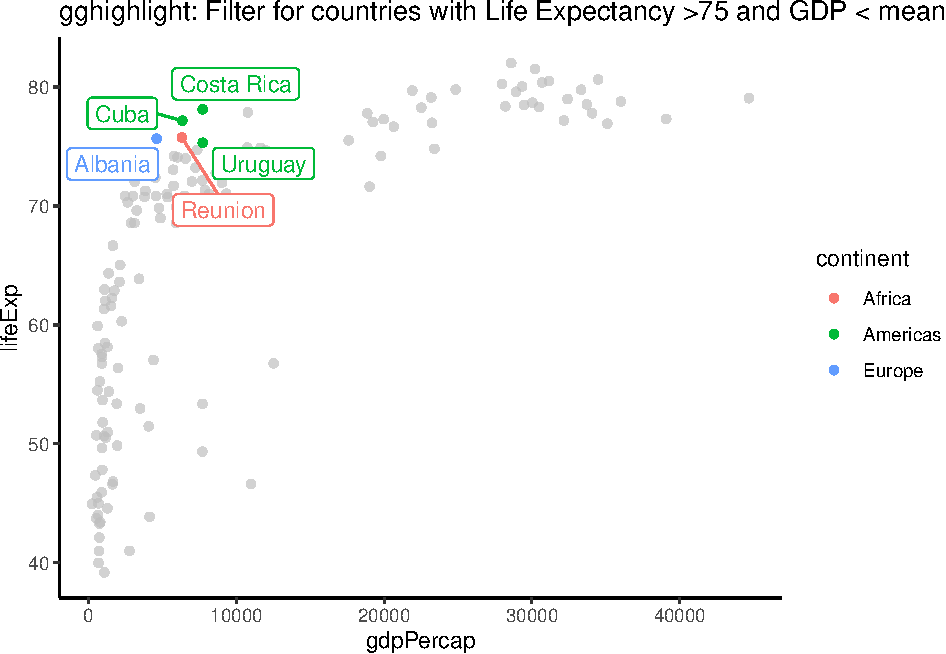
\includegraphics{cookbook_files/figure-latex/gghighlight-1.pdf}

\hypertarget{axis-font-size}{%
\section{Axis font size}\label{axis-font-size}}

\begin{Shaded}
\begin{Highlighting}[]
\CommentTok{# OPTION 1: theme(axis.text = element_text(size = 12, colour = "black"))}
\CommentTok{# OPTION 2: width and height arguments of ggsave()}

\KeywordTok{library}\NormalTok{(tidyverse)}
\KeywordTok{library}\NormalTok{(scales)}

\CommentTok{# made-up example data}
\NormalTok{mydata =}\StringTok{ }\KeywordTok{tibble}\NormalTok{(}\DataTypeTok{group    =} \KeywordTok{c}\NormalTok{(}\StringTok{"UMIC"}\NormalTok{, }\StringTok{"LMIC"}\NormalTok{, }\StringTok{"LIC"}\NormalTok{) }\OperatorTok\StringTok{ }\KeywordTok{rep}\NormalTok{(}\DataTypeTok{each =} \DecValTok{2}\NormalTok{),}
                \DataTypeTok{value    =} \DecValTok{1}\OperatorTok{:}\DecValTok{6}\NormalTok{, }
                \DataTypeTok{variable =} \KeywordTok{c}\NormalTok{(}\StringTok{"Yes"}\NormalTok{, }\StringTok{"No"}\NormalTok{) }\OperatorTok\StringTok{ }\KeywordTok{rep}\NormalTok{(}\DecValTok{3}\NormalTok{))}

\NormalTok{mydata }\OperatorTok\StringTok{ }
\StringTok{  }\KeywordTok{ggplot}\NormalTok{(}\KeywordTok{aes}\NormalTok{(}\DataTypeTok{x =}\NormalTok{ group, }\DataTypeTok{y =}\NormalTok{ value, }\DataTypeTok{fill =}\NormalTok{ variable)) }\OperatorTok{+}
\StringTok{  }\KeywordTok{geom_col}\NormalTok{(}\DataTypeTok{position =} \StringTok{"fill"}\NormalTok{) }\OperatorTok{+}
\StringTok{  }\KeywordTok{scale_y_continuous}\NormalTok{(}\DataTypeTok{labels =}\NormalTok{ percent, }\DataTypeTok{expand =} \KeywordTok{c}\NormalTok{(}\DecValTok{0}\NormalTok{, }\DecValTok{0}\NormalTok{)) }\OperatorTok{+}
\StringTok{  }\KeywordTok{theme_bw}\NormalTok{() }\OperatorTok{+}
\StringTok{  }\CommentTok{# OPTION 1: change font with theme()}
\StringTok{  }\KeywordTok{theme}\NormalTok{(}\DataTypeTok{axis.text  =} \KeywordTok{element_text}\NormalTok{(}\DataTypeTok{size =} \DecValTok{12}\NormalTok{, }\DataTypeTok{colour =} \StringTok{"black"}\NormalTok{),}
        \DataTypeTok{axis.title =} \KeywordTok{element_blank}\NormalTok{())}
\end{Highlighting}
\end{Shaded}

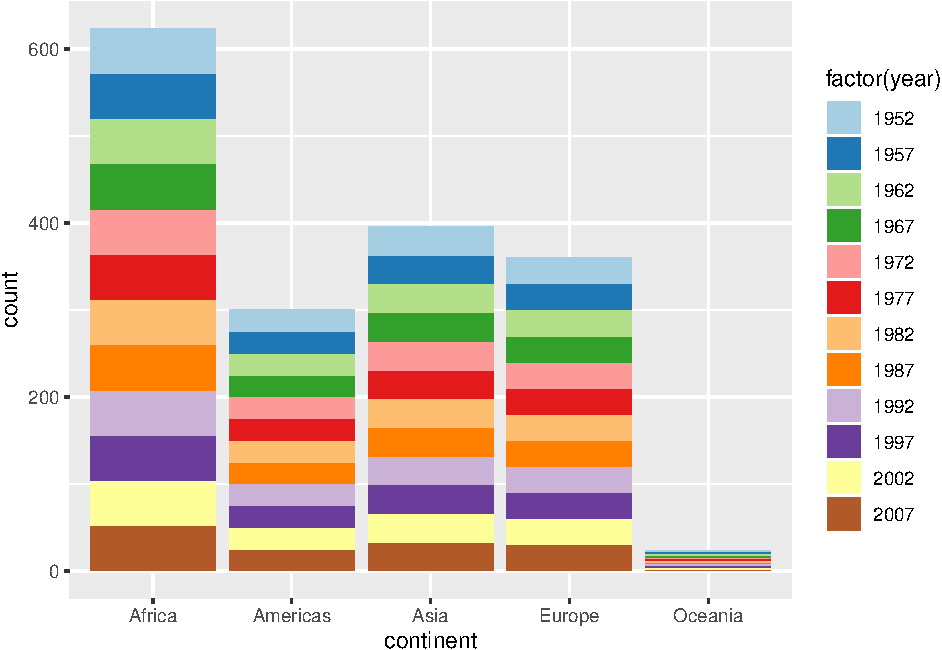
\includegraphics{cookbook_files/figure-latex/unnamed-chunk-37-1.pdf}

\begin{Shaded}
\begin{Highlighting}[]
\CommentTok{# OPTION 2: play around with export size. Since PDF will always have max resolution anyway}
\CommentTok{# but changing width and height modifies text size}
\NormalTok{mywidth  =}\StringTok{ }\DecValTok{5}
\NormalTok{myheight =}\StringTok{ }\DecValTok{4}
\CommentTok{#ggsave("barplot_5x4.pdf", width = mywidth, height = myheight)}

\NormalTok{mywidth  =}\StringTok{ }\DecValTok{10}
\NormalTok{myheight =}\StringTok{ }\DecValTok{8}
\CommentTok{#ggsave("barplot_10x8.pdf", width = mywidth, height = myheight)}
\end{Highlighting}
\end{Shaded}

Same plot 5x4 inches vs 10x8 inches:

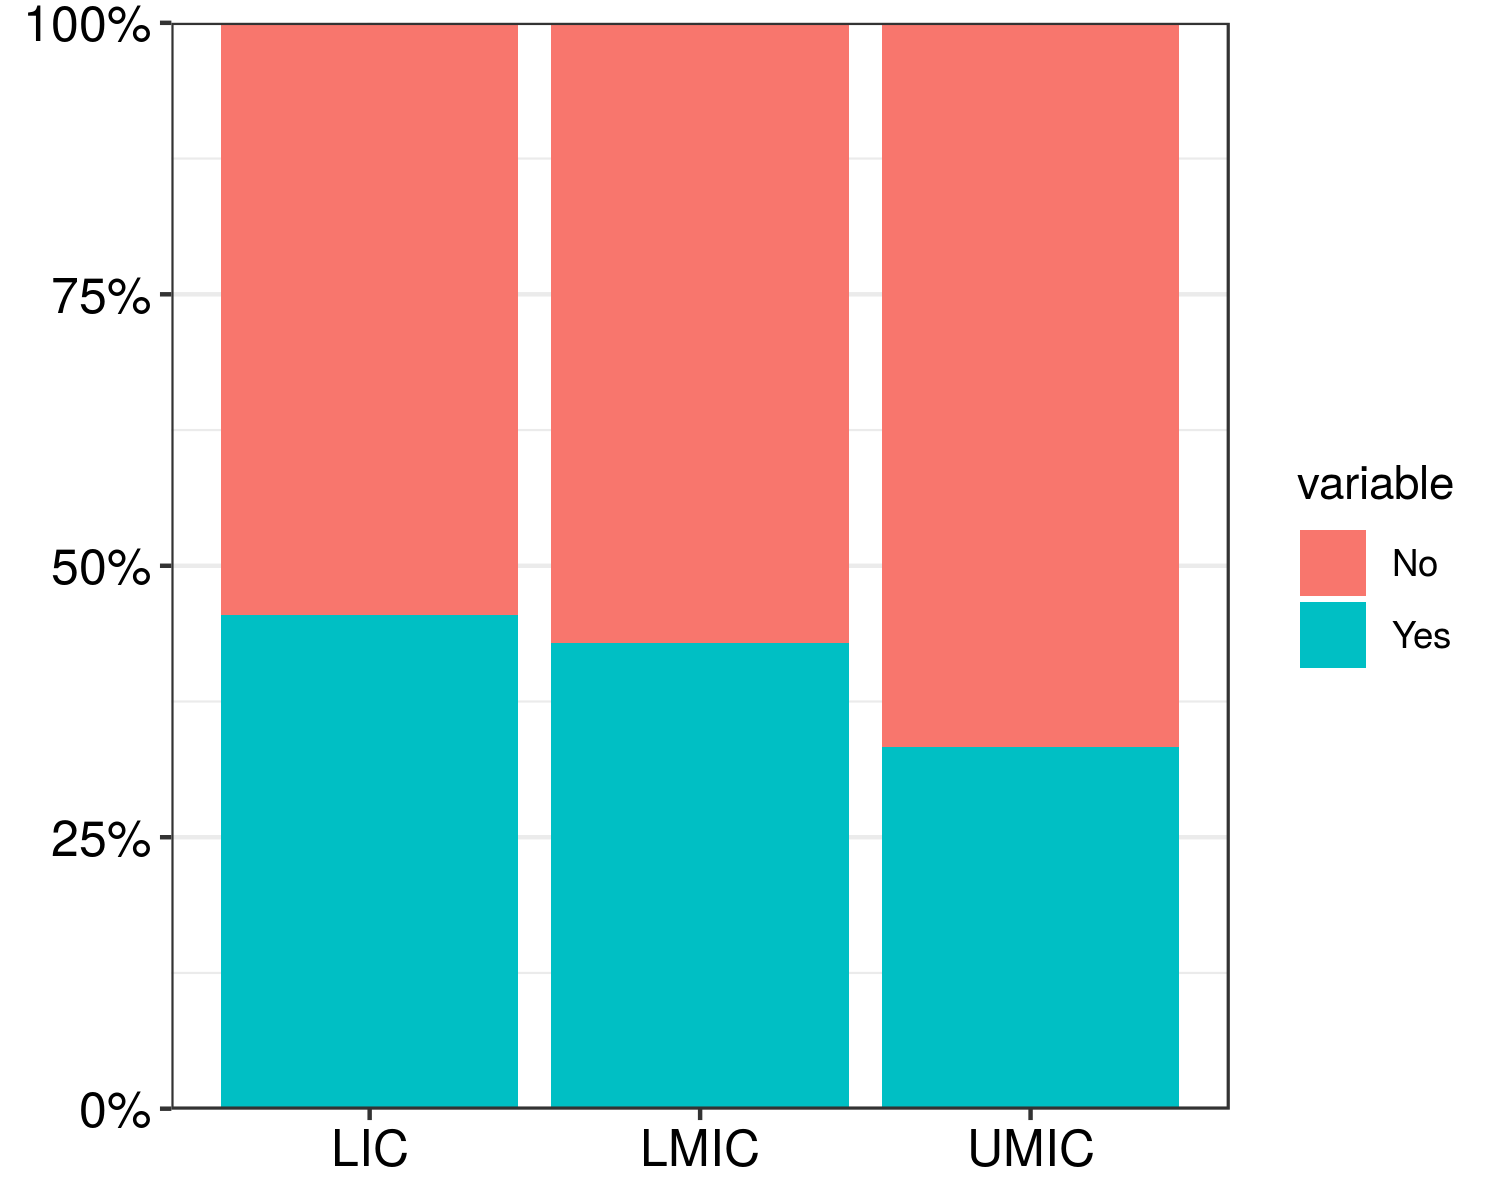
\includegraphics[width=0.5\linewidth]{/home/rots/cookbook/img/barplot_5x4}
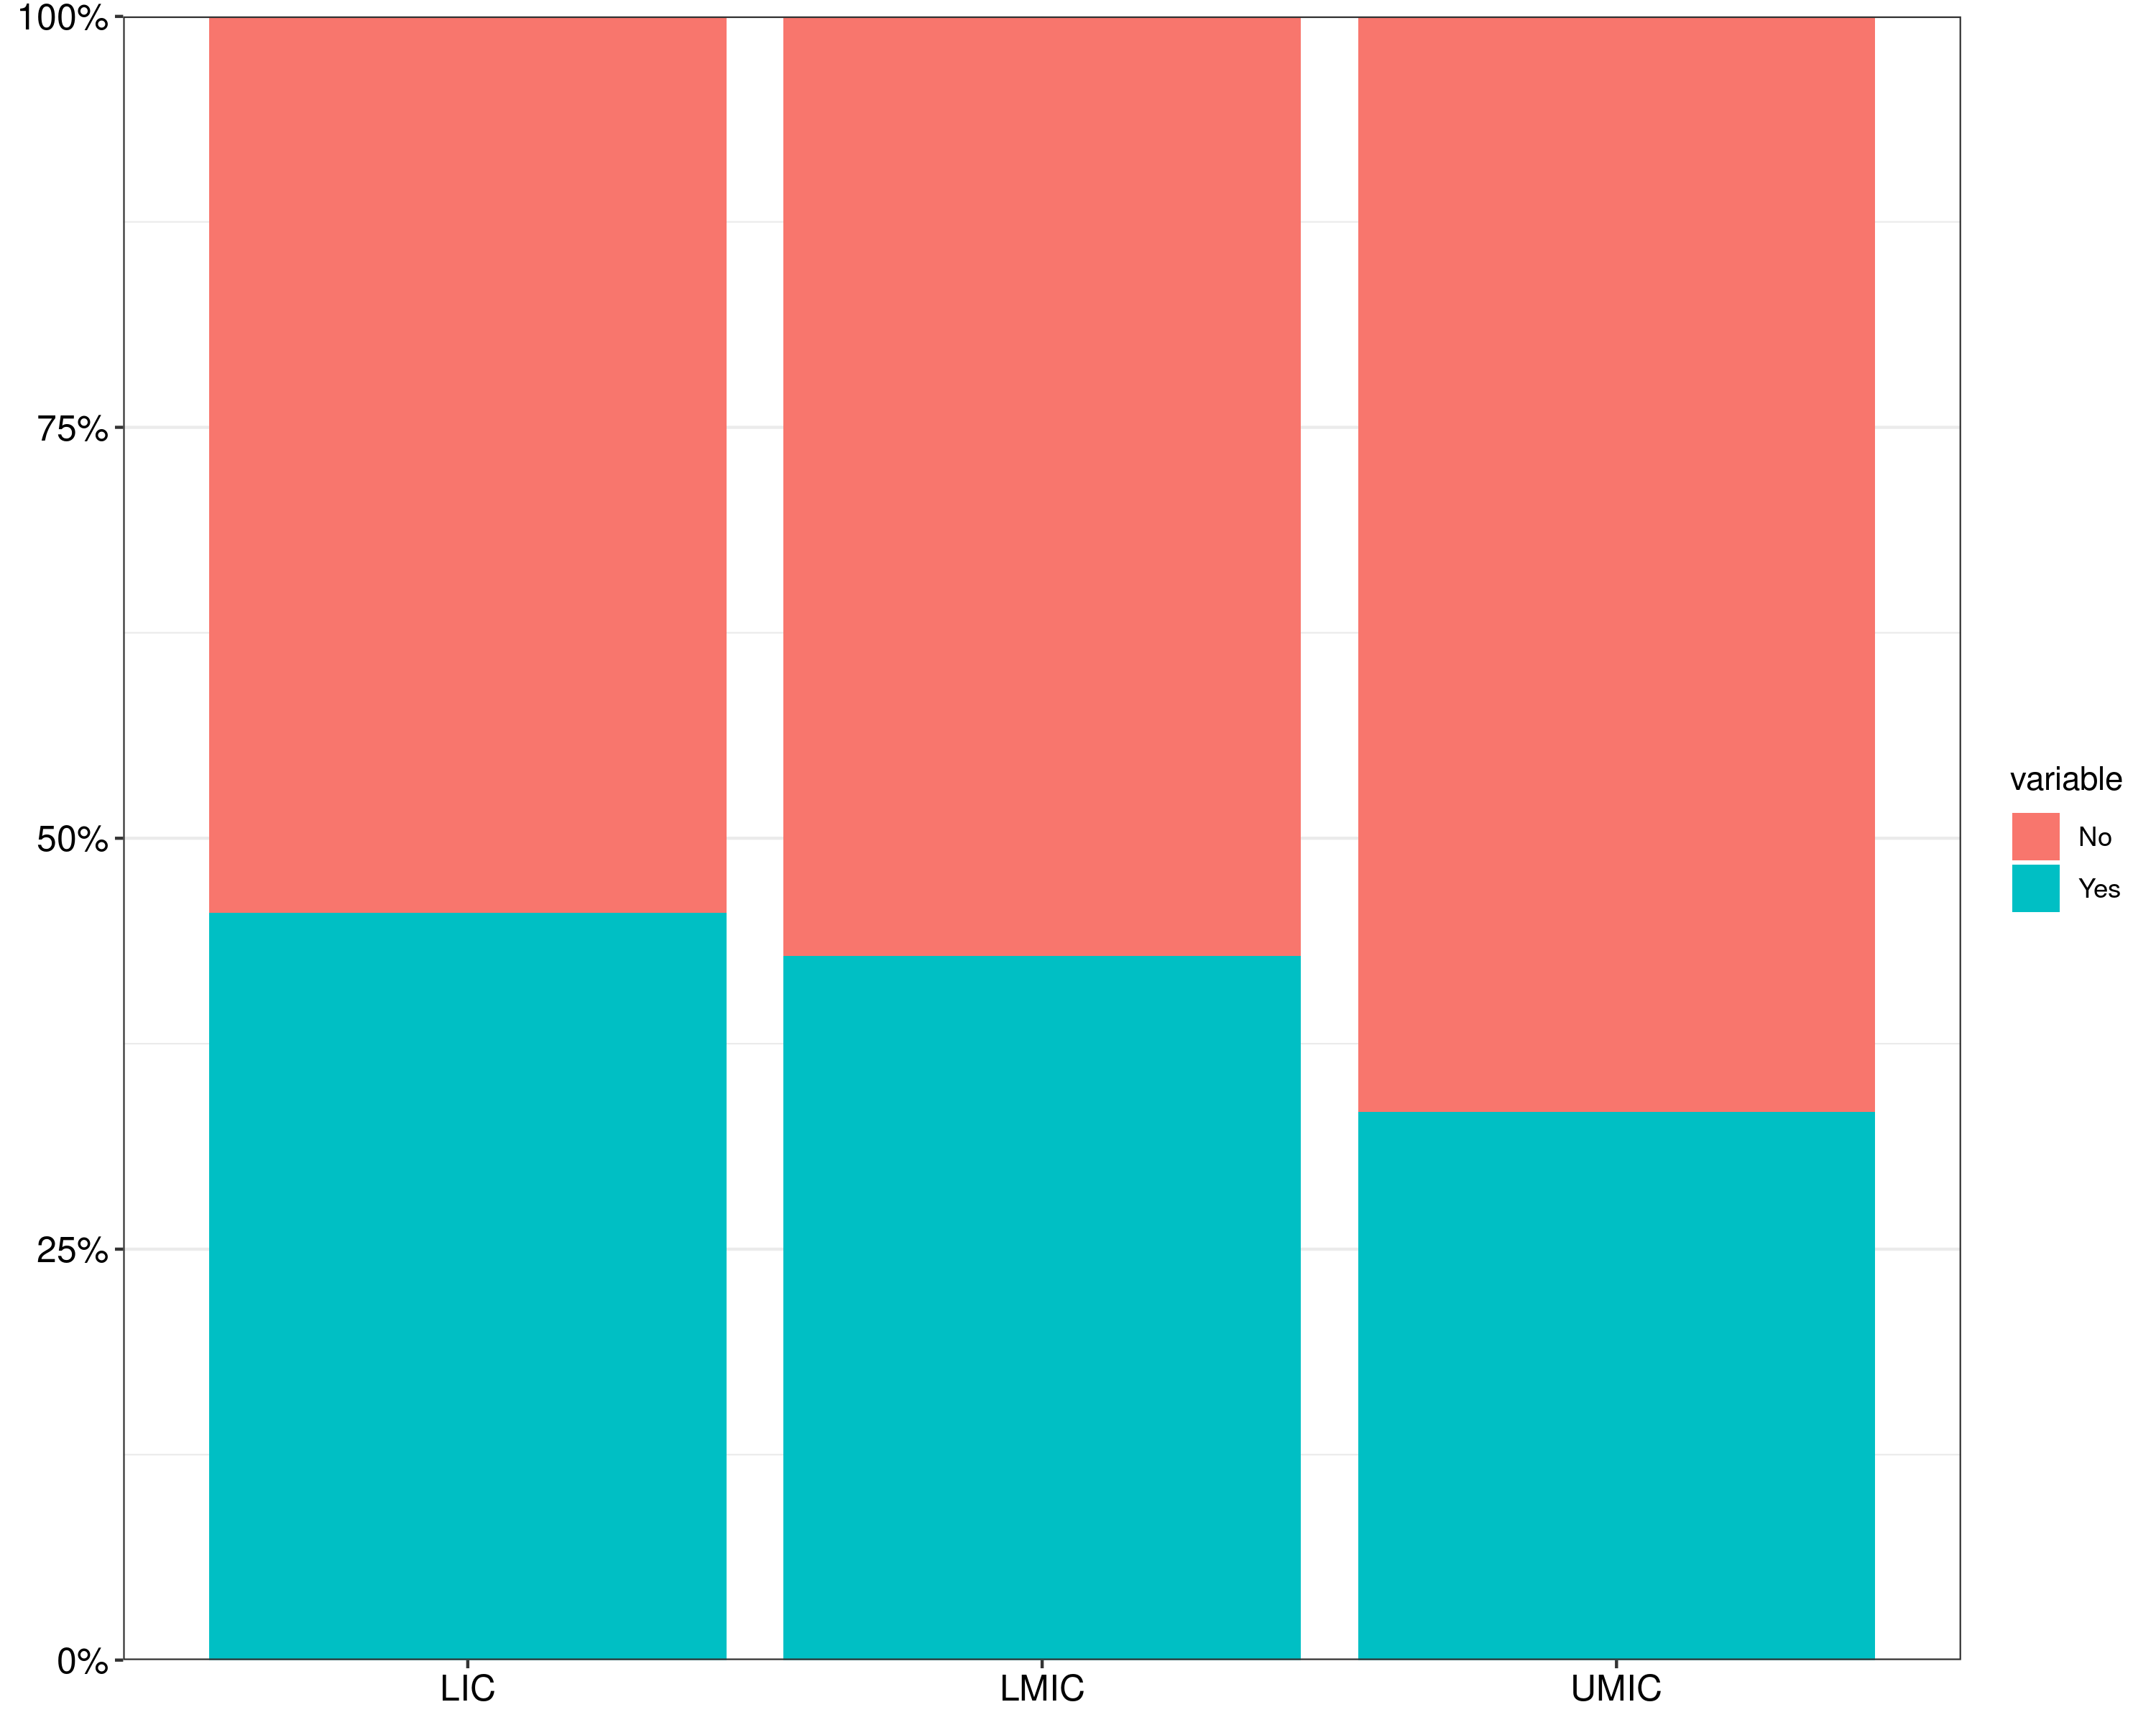
\includegraphics[width=0.5\linewidth]{/home/rots/cookbook/img/barplot_10x8}

\hypertarget{genomics}{%
\chapter{Genomics}\label{genomics}}

\hypertarget{single-cell-analysis}{%
\section{Single Cell Analysis}\label{single-cell-analysis}}

\hypertarget{minimising-the-size-of-a-seurat-object}{%
\subsection{Minimising the size of a Seurat
Object}\label{minimising-the-size-of-a-seurat-object}}

Single cell analyses are ofetn collated in Seurat objects which can be
huge. We reduced the size of our Seurat object by pulling the relevant
sections using the code below reducing the object to \textless{}20\% of
its original size. This works by only including the sparse matrices.
This is not a workable example, but the PBMC dataset could be used if
necessary.

\begin{Shaded}
\begin{Highlighting}[]
\CommentTok{#library(Seurat)}
\CommentTok{#library(dplyr)}


\CommentTok{#Load in the data}

\NormalTok{pathtoglobaldata <-}\StringTok{"mac_shiny/data/Global_sc_object"}
\NormalTok{object_global<-}\KeywordTok{readRDS}\NormalTok{(pathtoglobaldata)}


\CommentTok{# Get sparse assay data}
\NormalTok{sizetest_global<-}\KeywordTok{GetAssayData}\NormalTok{(}\DataTypeTok{object =}\NormalTok{ object_global, }\DataTypeTok{slot =} \StringTok{"data"}\NormalTok{) }\CommentTok{# counts don’t work, scaled breaks my pc with memory errors, not sure it matters that much}
\NormalTok{object_global_small<-}\StringTok{ }\KeywordTok{CreateSeuratObject}\NormalTok{(sizetest_global)}

\CommentTok{# Add in classifications. }

\NormalTok{object_global_small}\OperatorTok{@}\NormalTok{reductions}\OperatorTok{$}\NormalTok{tsne<-object_global}\OperatorTok{@}\NormalTok{reductions}\OperatorTok{$}\NormalTok{tsne }\CommentTok{# reduction embeddings for tsnegraph}
\NormalTok{object_global_small}\OperatorTok{$}\NormalTok{Phenotype<-}\StringTok{ }\NormalTok{object_global}\OperatorTok{$}\NormalTok{Phenotype}

\NormalTok{object_global_small}\OperatorTok{@}\NormalTok{meta.data}\OperatorTok{$}\NormalTok{final_classification<-}\StringTok{ }\NormalTok{object_global}\OperatorTok{@}\NormalTok{meta.data}\OperatorTok{$}\NormalTok{final_classification}
\NormalTok{object_global_small}\OperatorTok{$}\NormalTok{final_classificaiton<-}\StringTok{ }\NormalTok{object_global}\OperatorTok{$}\NormalTok{final_classification }\CommentTok{#cell classifications}
\KeywordTok{Idents}\NormalTok{(}\DataTypeTok{object =}\NormalTok{ object_global_small) <-}\StringTok{ "final_classificaiton"} \CommentTok{#set forever}


\CommentTok{#same}
\KeywordTok{saveRDS}\NormalTok{(object_global_small,}\StringTok{"mac_shiny/data/global_object_sml"}\NormalTok{)}
\end{Highlighting}
\end{Shaded}

\hypertarget{programming-in-rlang}{%
\chapter{Programming in rlang}\label{programming-in-rlang}}

\hypertarget{rlang}{%
\section{rlang}\label{rlang}}

\hypertarget{what-is-rlang}{%
\subsection{What is rlang?}\label{what-is-rlang}}

rlang is a low-level programming API for R which the tidyverse uses
(meaning it speaks to R in as R like way as possible, rather than a
`high-level' - high level is more user orientated and interpretable). It
enables you to extend what the tidyverse can do and adapt it for your
own uses. It's particularly good to use if you're doing lots of more
`programming' type R work, for example, building a package, making a
complex shiny app or writing functions. It might also be handy if you're
doing lots of big data manipulation and want to manipulate different
datasets in the same way, for example.

In this chapter we'll discuss some uses of it.

\hypertarget{dynamic-calling-of-variables-using-dplyr}{%
\subsection{Dynamic calling of variables using
dplyr}\label{dynamic-calling-of-variables-using-dplyr}}

In this example, say we have a tibble of variables, but we want to apply
dynamic changes to it (so we feed R a variable, that can change, either
using another function like \texttt{purr::map} or in a ShinyApp). In
this instance, specifying each variable and each different possible
consequence using different logical functions would take forever and be
very clunky. So we can use rlang to simply put a dynamic variable/object
through the same function.

We'll use an example where we want to summarise by different outcomes in
a dynamic way.

\begin{Shaded}
\begin{Highlighting}[]
\KeywordTok{library}\NormalTok{(tidyverse)}
\CommentTok{#Make data - here nonsense numbers on deaths per 100k from guns say}

\NormalTok{example_data =}\StringTok{ }\KeywordTok{tibble}\NormalTok{(}\DataTypeTok{countries =} \KeywordTok{c}\NormalTok{(}\StringTok{'UK'}\NormalTok{, }\StringTok{'USA'}\NormalTok{, }\StringTok{'Pakistan'}\NormalTok{, }\StringTok{'Mexico'}\NormalTok{, }\StringTok{'Ireland'}\NormalTok{, }\StringTok{'Estonia'}\NormalTok{),}
                      \DataTypeTok{region =} \KeywordTok{c}\NormalTok{(}\StringTok{'Europe'}\NormalTok{, }\StringTok{'Americas'}\NormalTok{, }\StringTok{'Asia'}\NormalTok{, }\StringTok{'Americas'}\NormalTok{, }\StringTok{'Europe'}\NormalTok{, }\StringTok{'Europe'}\NormalTok{),}
                      \DataTypeTok{Death_from_guns =} \KeywordTok{c}\NormalTok{(}\DecValTok{1}\NormalTok{, }\DecValTok{200}\NormalTok{, }\DecValTok{150}\NormalTok{, }\DecValTok{450}\NormalTok{, }\DecValTok{3}\NormalTok{, }\FloatTok{3.5}\NormalTok{),}
                      \DataTypeTok{Death_from_smoking =} \KeywordTok{c}\NormalTok{(}\DecValTok{100}\NormalTok{, }\DecValTok{300}\NormalTok{, }\DecValTok{140}\NormalTok{, }\DecValTok{150}\NormalTok{, }\DecValTok{120}\NormalTok{, }\DecValTok{300}\NormalTok{))}


\CommentTok{#example function for summarising using dynamic variables and bang bangs}
\CommentTok{#note metric must be numeric}
\NormalTok{summarise_feature =}\StringTok{ }\ControlFlowTok{function}\NormalTok{(df, col_var, ...)\{}
  \KeywordTok{require}\NormalTok{(tidyverse)}
  
\NormalTok{  wurly_curly =}\StringTok{ }\ControlFlowTok{function}\NormalTok{(.)\{}\CommentTok{#The wurly_curly function makes things nicer}
  \KeywordTok{require}\NormalTok{(rlang)}
  \OperatorTok{!!}\KeywordTok{quo_name}\NormalTok{(}\KeywordTok{enquo}\NormalTok{(.))\}}

\NormalTok{  summary_nm_sum <-}\StringTok{ }\KeywordTok{paste0}\NormalTok{(}\StringTok{"metric_"}\NormalTok{, }\KeywordTok{wurly_curly}\NormalTok{(col_var))}\CommentTok{#The new LHS variable must have a different name from that on the RHS}

\NormalTok{  df }\OperatorTok
\StringTok{    }\KeywordTok{group_by}\NormalTok{(...) }\OperatorTok\StringTok{ }
\StringTok{    }\KeywordTok{summarise}\NormalTok{(}\OperatorTok{!!}\NormalTok{summary_nm_sum }\OperatorTok{:}\ErrorTok{=}\StringTok{ }\KeywordTok{sum}\NormalTok{(\{\{col_var\}\}))}
\NormalTok{\}}


\CommentTok{#output new variable}
\NormalTok{example_data }\OperatorTok\StringTok{ }
\StringTok{  }\KeywordTok{summarise_feature}\NormalTok{(Death_from_guns, region) }

\CommentTok{#How to dynamically change names using mutate and rlang}
\CommentTok{#Bang bang variables into mutate/tidyverse(so they can be dynamically changed)}

\CommentTok{#Select metric}
\NormalTok{metric =}\StringTok{ 'metric_Death_from_guns'} \CommentTok{#example but can be any named column}

\NormalTok{metric_mutate =}\StringTok{ }\KeywordTok{paste0}\NormalTok{(}\StringTok{'prefix_'}\NormalTok{, metric) }\CommentTok{#some reason doesn't take these within the mutate function so has to be outside}

\NormalTok{example_data }\OperatorTok\StringTok{ }
\StringTok{  }\KeywordTok{summarise_feature}\NormalTok{(Death_from_guns, region) }\OperatorTok\StringTok{ }
\StringTok{  }\KeywordTok{mutate}\NormalTok{(}\OperatorTok{!!}\NormalTok{metric_mutate }\OperatorTok{:}\ErrorTok{=}\StringTok{ }\OperatorTok{!!}\NormalTok{rlang}\OperatorTok{::}\KeywordTok{sym}\NormalTok{(metric) }\OperatorTok{*}\StringTok{ }\DecValTok{2}\NormalTok{)}\CommentTok{#apply arbitary multiplication by two}
\end{Highlighting}
\end{Shaded}

\bibliography{book.bib,packages.bib}


\end{document}
